\documentclass[12pt,a4paper]{article}
\usepackage[utf8]{inputenc}
\usepackage[catalan]{babel}
\usepackage{graphicx}
\usepackage{geometry}
\usepackage{fancyhdr}
\usepackage{tabularx}
\usepackage{lastpage}
\usepackage{enumitem}
\usepackage{amsmath}
\usepackage{float} % Per gestionar millor la posició de les imatges

% 1. MARGES I CAPÇALERA
\geometry{top=4cm, bottom=3cm, left=2cm, right=2cm, headheight=2.5cm}

\pagestyle{fancy}
\fancyhf{}
% Assegura't que tens els fitxers d'imatge o comenta aquestes línies si no els tens
\fancyhead[L]{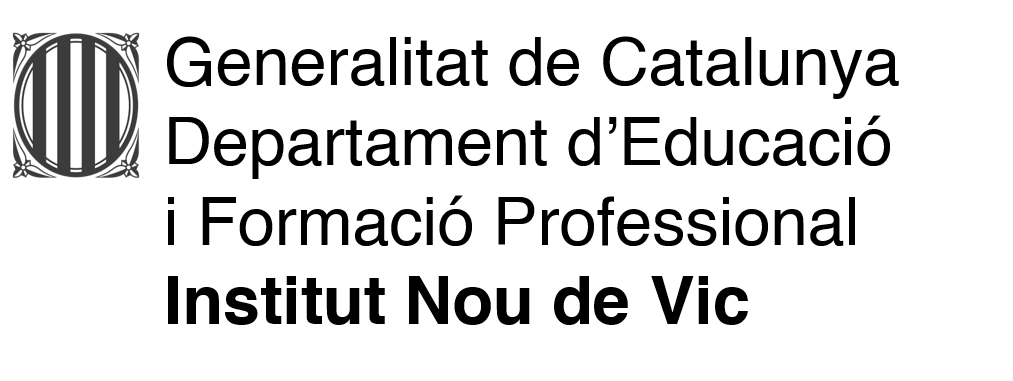
\includegraphics[height=1.8cm]{Logo_Departament.png}} 
\fancyhead[R]{
\includegraphics[height=1.8cm]{Logo_Institut.png}}

\fancyfoot[L]{}
\fancyfoot[C]{Pàgina \thepage\ de \pageref{LastPage}}
\fancyfoot[R]{}

\renewcommand{\headrulewidth}{0.4pt}

\begin{document}

% --- CAPÇALERA D'IDENTIFICACIÓ ---
\begingroup
\renewcommand{\arraystretch}{2.2}
\begin{tabularx}{\textwidth}{|X|p{4cm}|}
    \hline
    \textbf{Nom i cognoms:} & \textbf{Grup:} \\ \hline
    \textbf{Activitat:} Geometria Analítica - Rectes & \textbf{Data:} \\ \hline
\end{tabularx}
\endgroup

\vspace{0.8cm}

\begin{center}
    {\Large \textbf{RESOLUCIÓ D'EXERCICIS DE RECTES}}
\end{center}

% --- EXERCICI 20 ---
\section*{Exercici 20 Activitats Finals}
\textbf{Un paral·lelogram $OABC$ té els seus vèrtexs en els punts $O(0, 0)$, $A(3, 1)$ i $C(1, 2)$. Calcula les coordenades del vèrtex $B$ i l'àrea del paral·lelogram.}

\vspace{0.5cm}

Comencem representant els tres punts inicials al pla cartesià:

\begin{figure}[H]
    \centering
    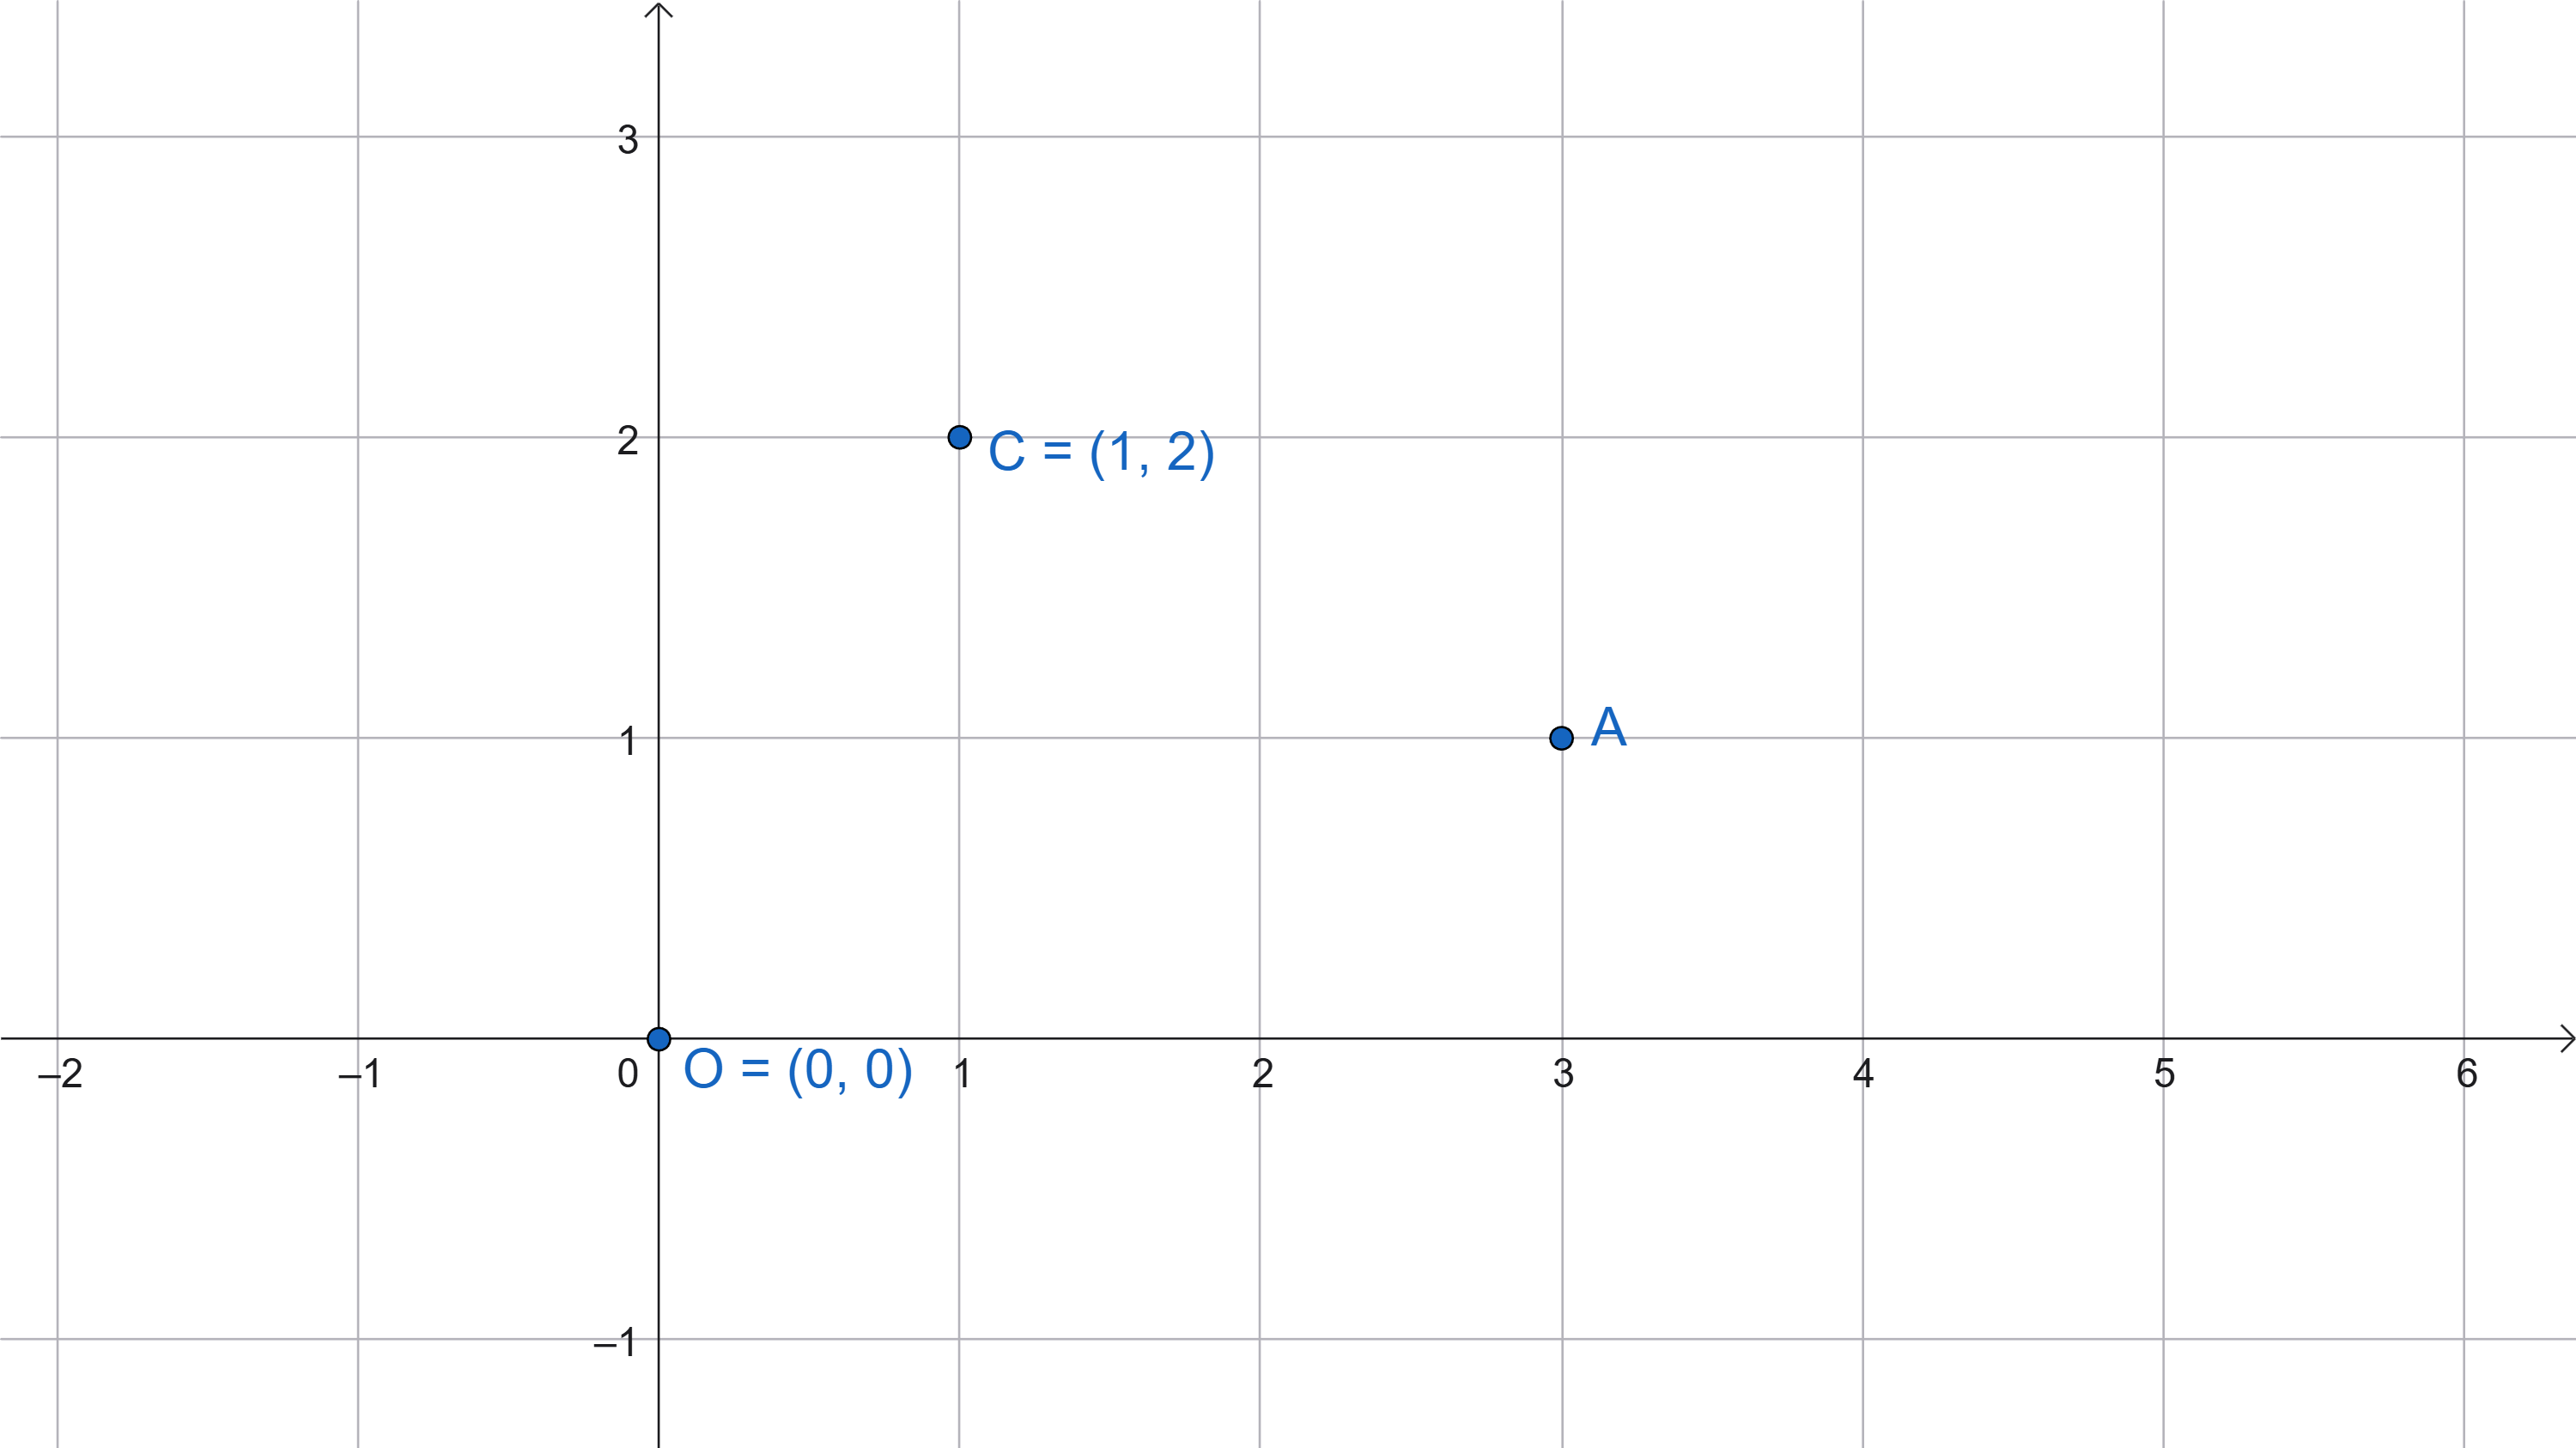
\includegraphics[width=0.7\textwidth]{Rectes al pla - 20 AF paral·lelogram àrea_1.png}
    \caption{Punts donats de l'enunciat.}
\end{figure}

\subsection*{1. Càlcul del vèrtex B}

En un paral·lelogram, els costats oposats són paral·lels i de la mateixa longitud. Això vol dir que els vectors dels costats oposats són equipol·lents (iguals).
Per arribar al punt $B$, podem sumar al punt $C$ el vector $\vec{OA}$, o bé sumar els dos vectors directors des de l'origen:
\[ \vec{OB} = \vec{OA} + \vec{OC} \]

\begin{enumerate}
    \item \textbf{Definim els vectors:}
    \[ \vec{OA} = A - O = (3, 1) - (0, 0) = (3, 1) \]
    \[ \vec{OC} = C - O = (1, 2) - (0, 0) = (1, 2) \]

    \begin{figure}[H]
        \centering
        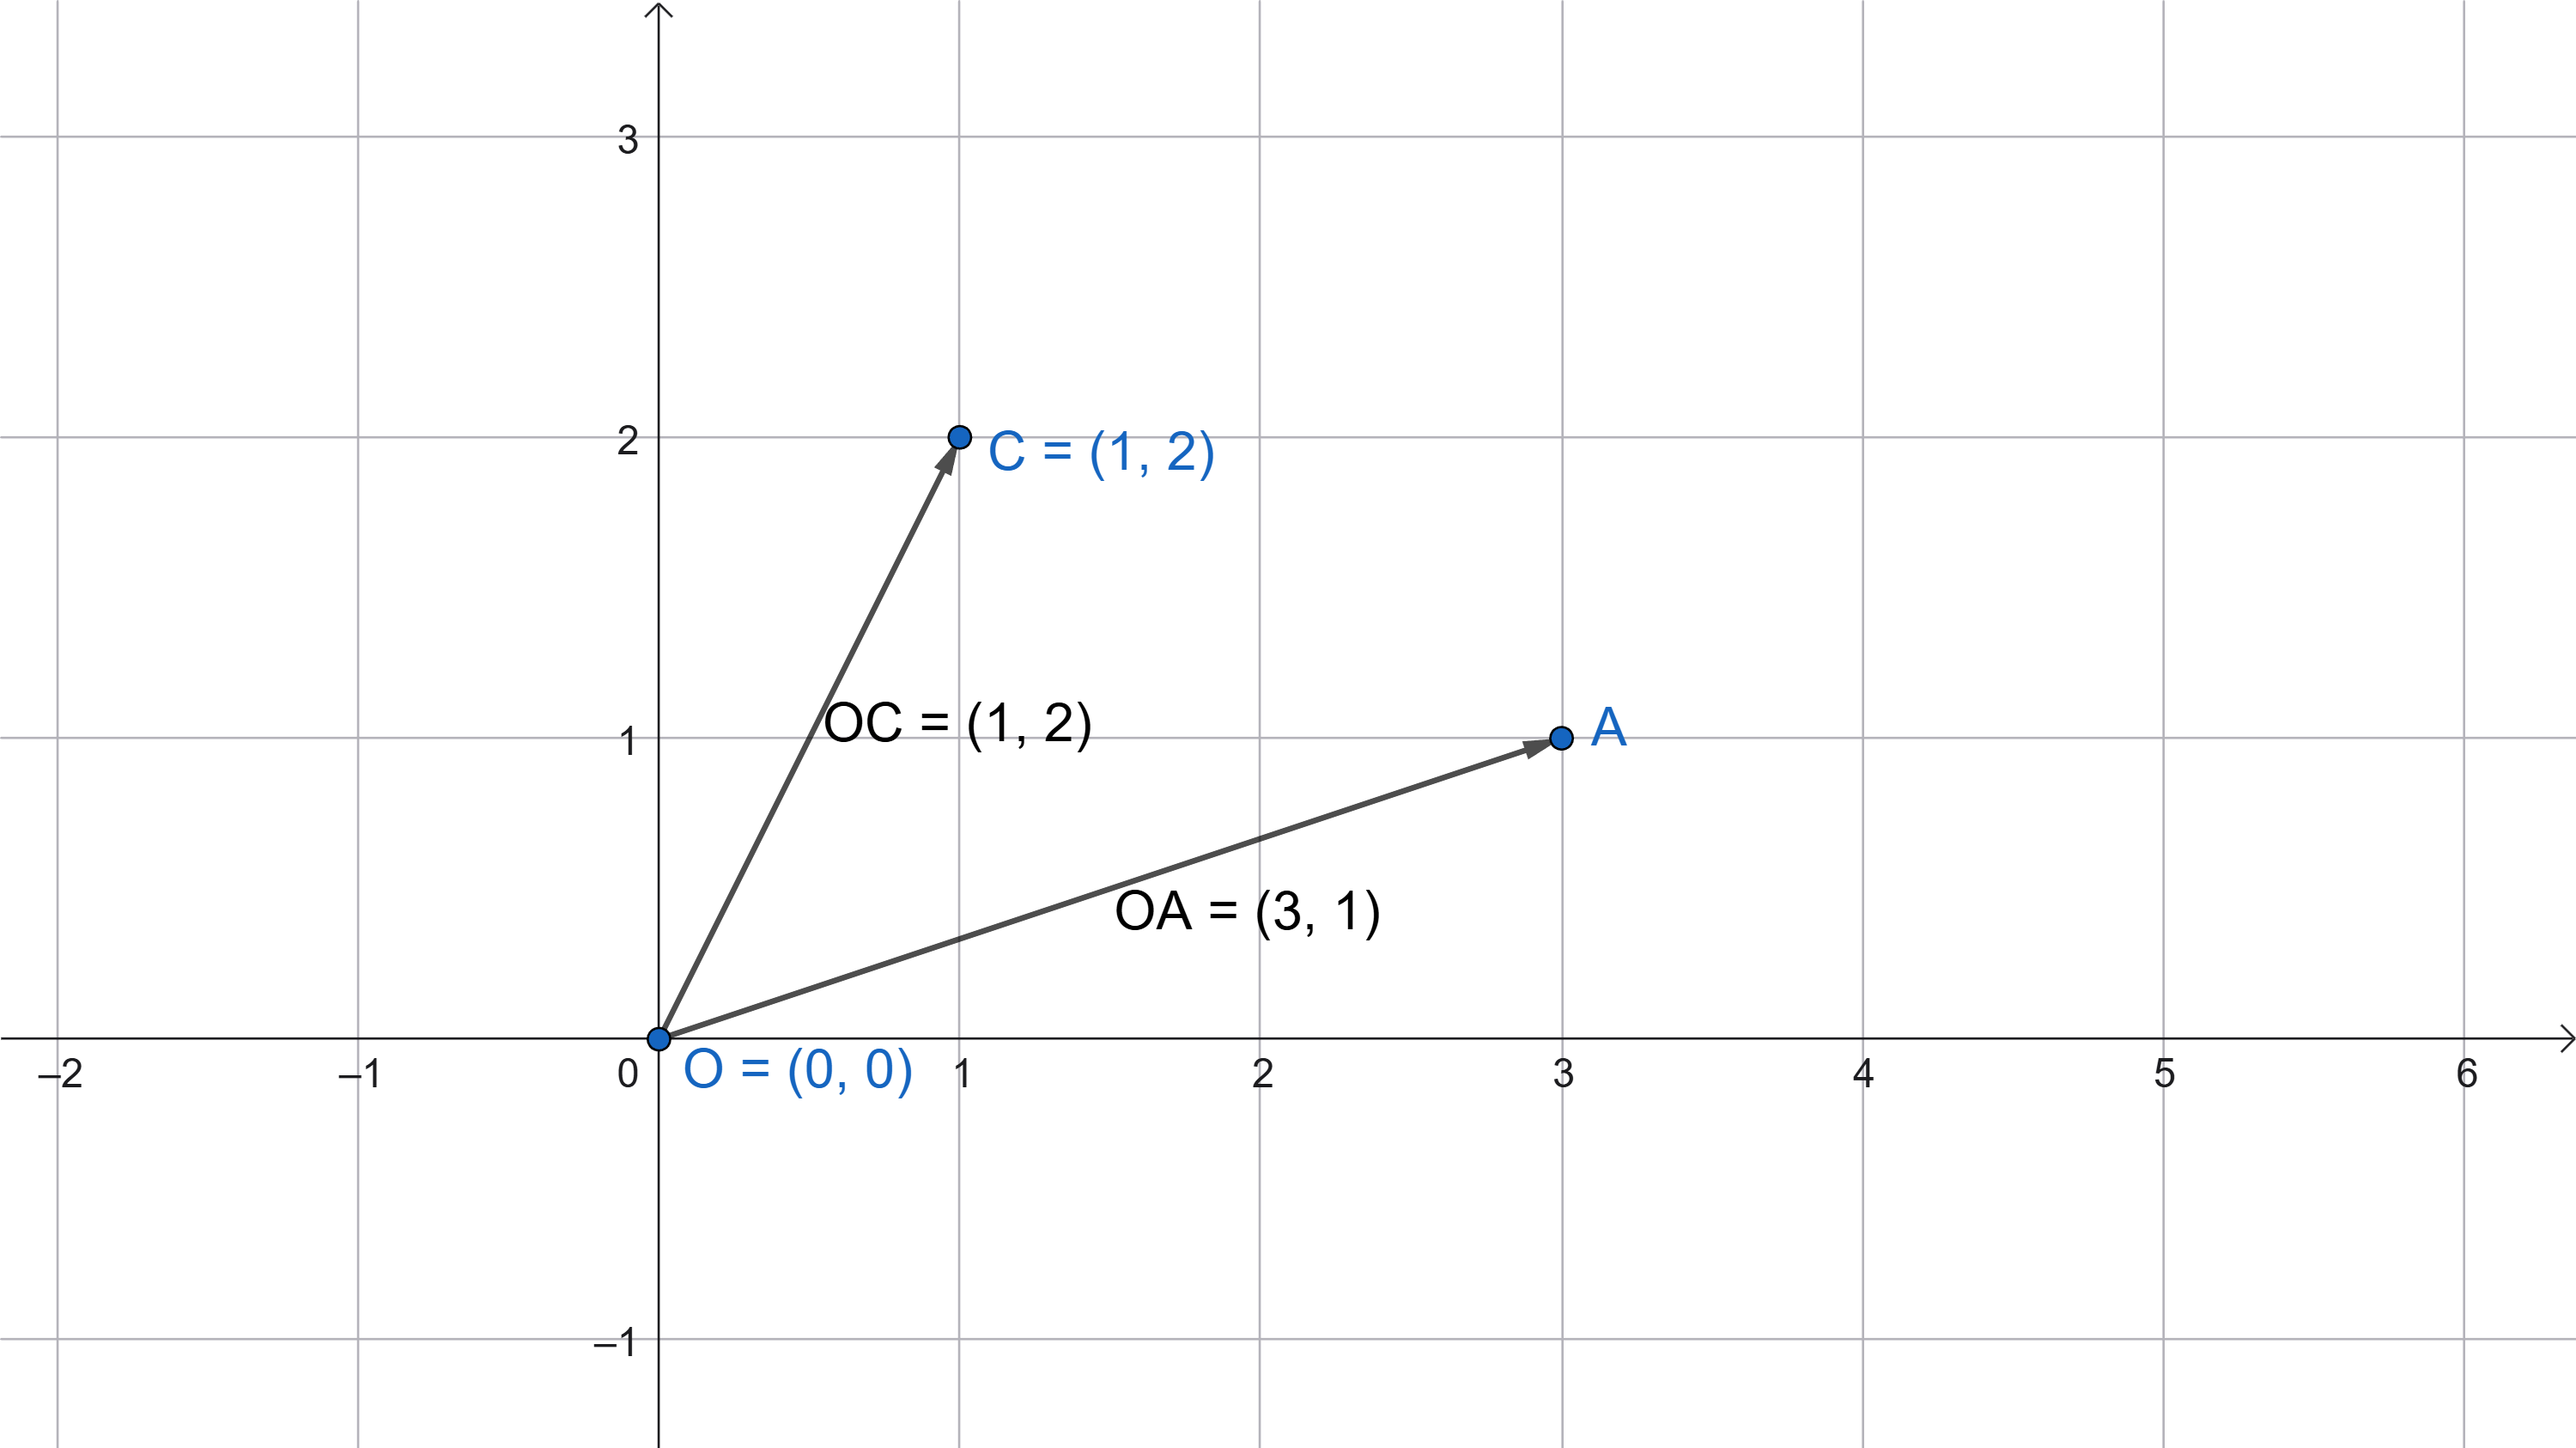
\includegraphics[width=0.7\textwidth]{Rectes al pla - 20 AF paral·lelogram àrea_2.png}
        \caption{Vectors que defineixen els costats del paral·lelogram.}
    \end{figure}

    \item \textbf{Calculem B:}
    \[ B = O + \vec{OA} + \vec{OC} = (0,0) + (3, 1) + (1, 2) = (4, 3) \]
    
    Les coordenades del vèrtex $B$ són $\boxed{B(4, 3)}$.
\end{enumerate}

\begin{figure}[H]
    \centering
    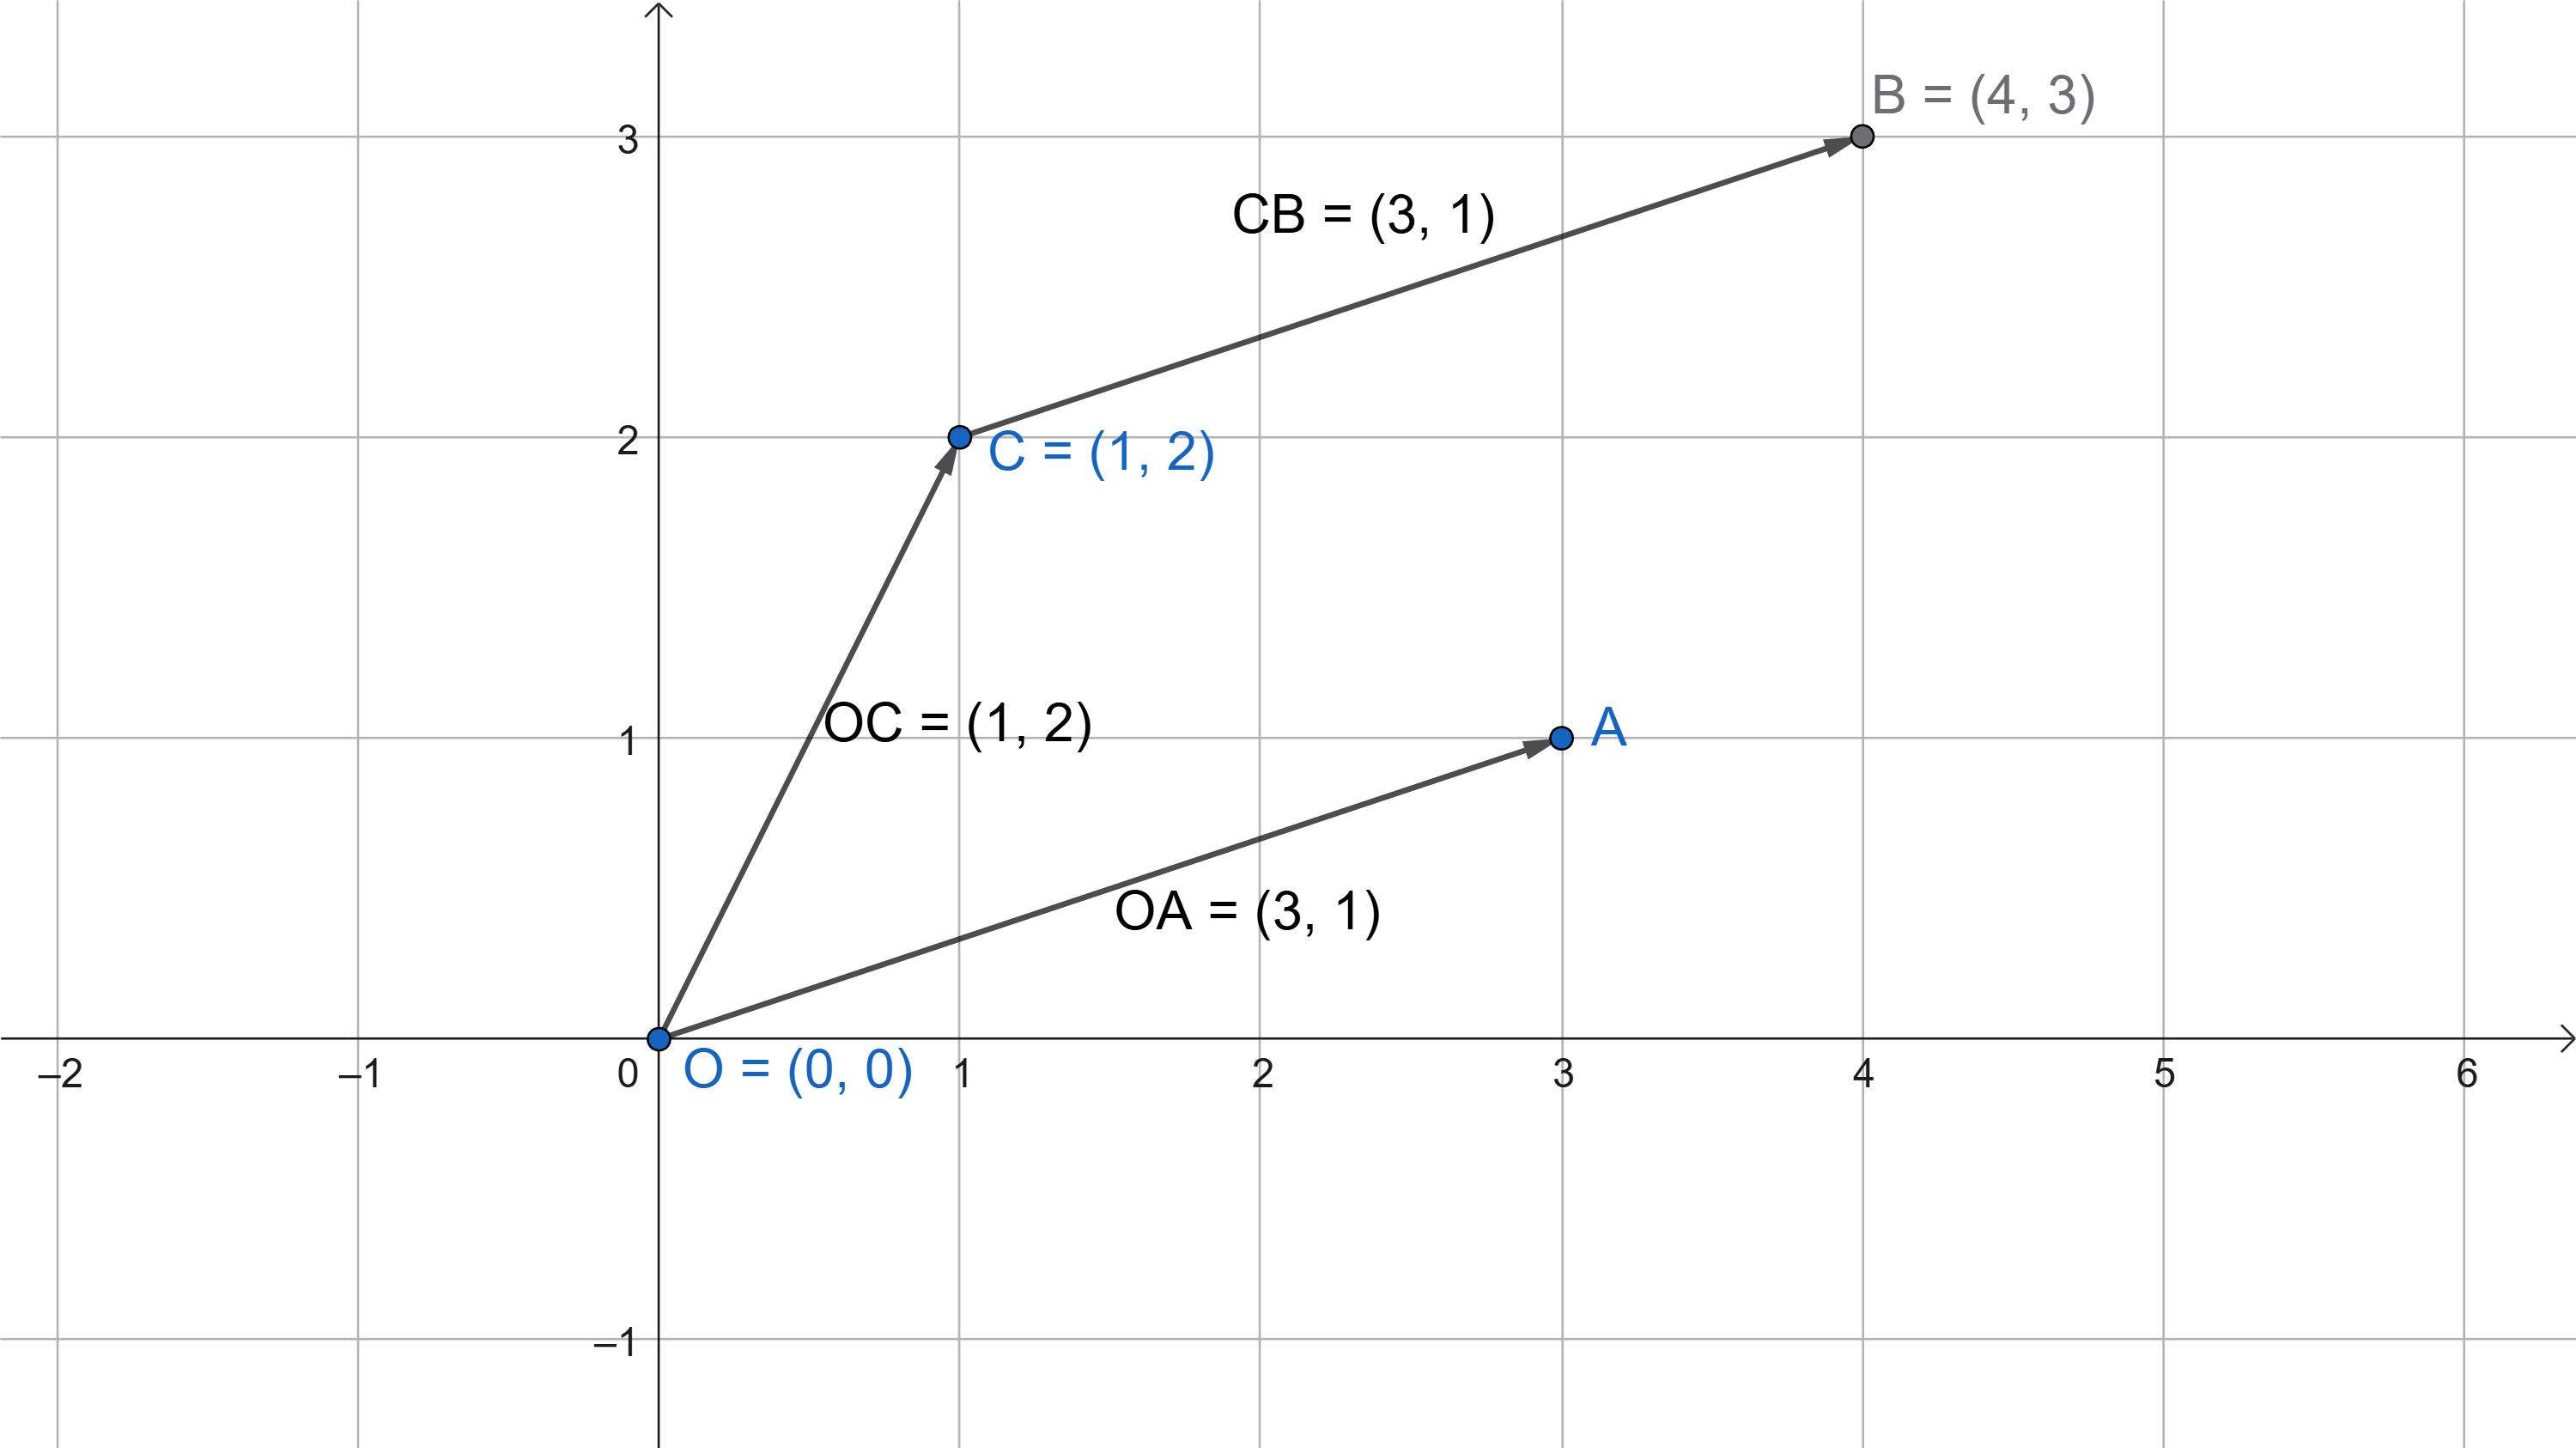
\includegraphics[width=0.7\textwidth]{Rectes al pla - 20 AF paral·lelogram àrea_3.png}
    \caption{Representació del paral·lelogram complet.}
\end{figure}

\newpage

\subsection*{2. Càlcul de l'àrea}

Per calcular l'àrea d'un paral·lelogram, utilitzem la fórmula:
\[ \text{Àrea} = \text{base} \times \text{altura} \]

En geometria analítica, podem interpretar l'àrea transformant el paral·lelogram en un rectangle equivalent. Si tracem l'altura des del vèrtex $C$ fins a la base $OA$, el triangle que "tallem" d'un costat és exactament el que falta a l'altre costat.
\begin{figure}[H]
    \centering
    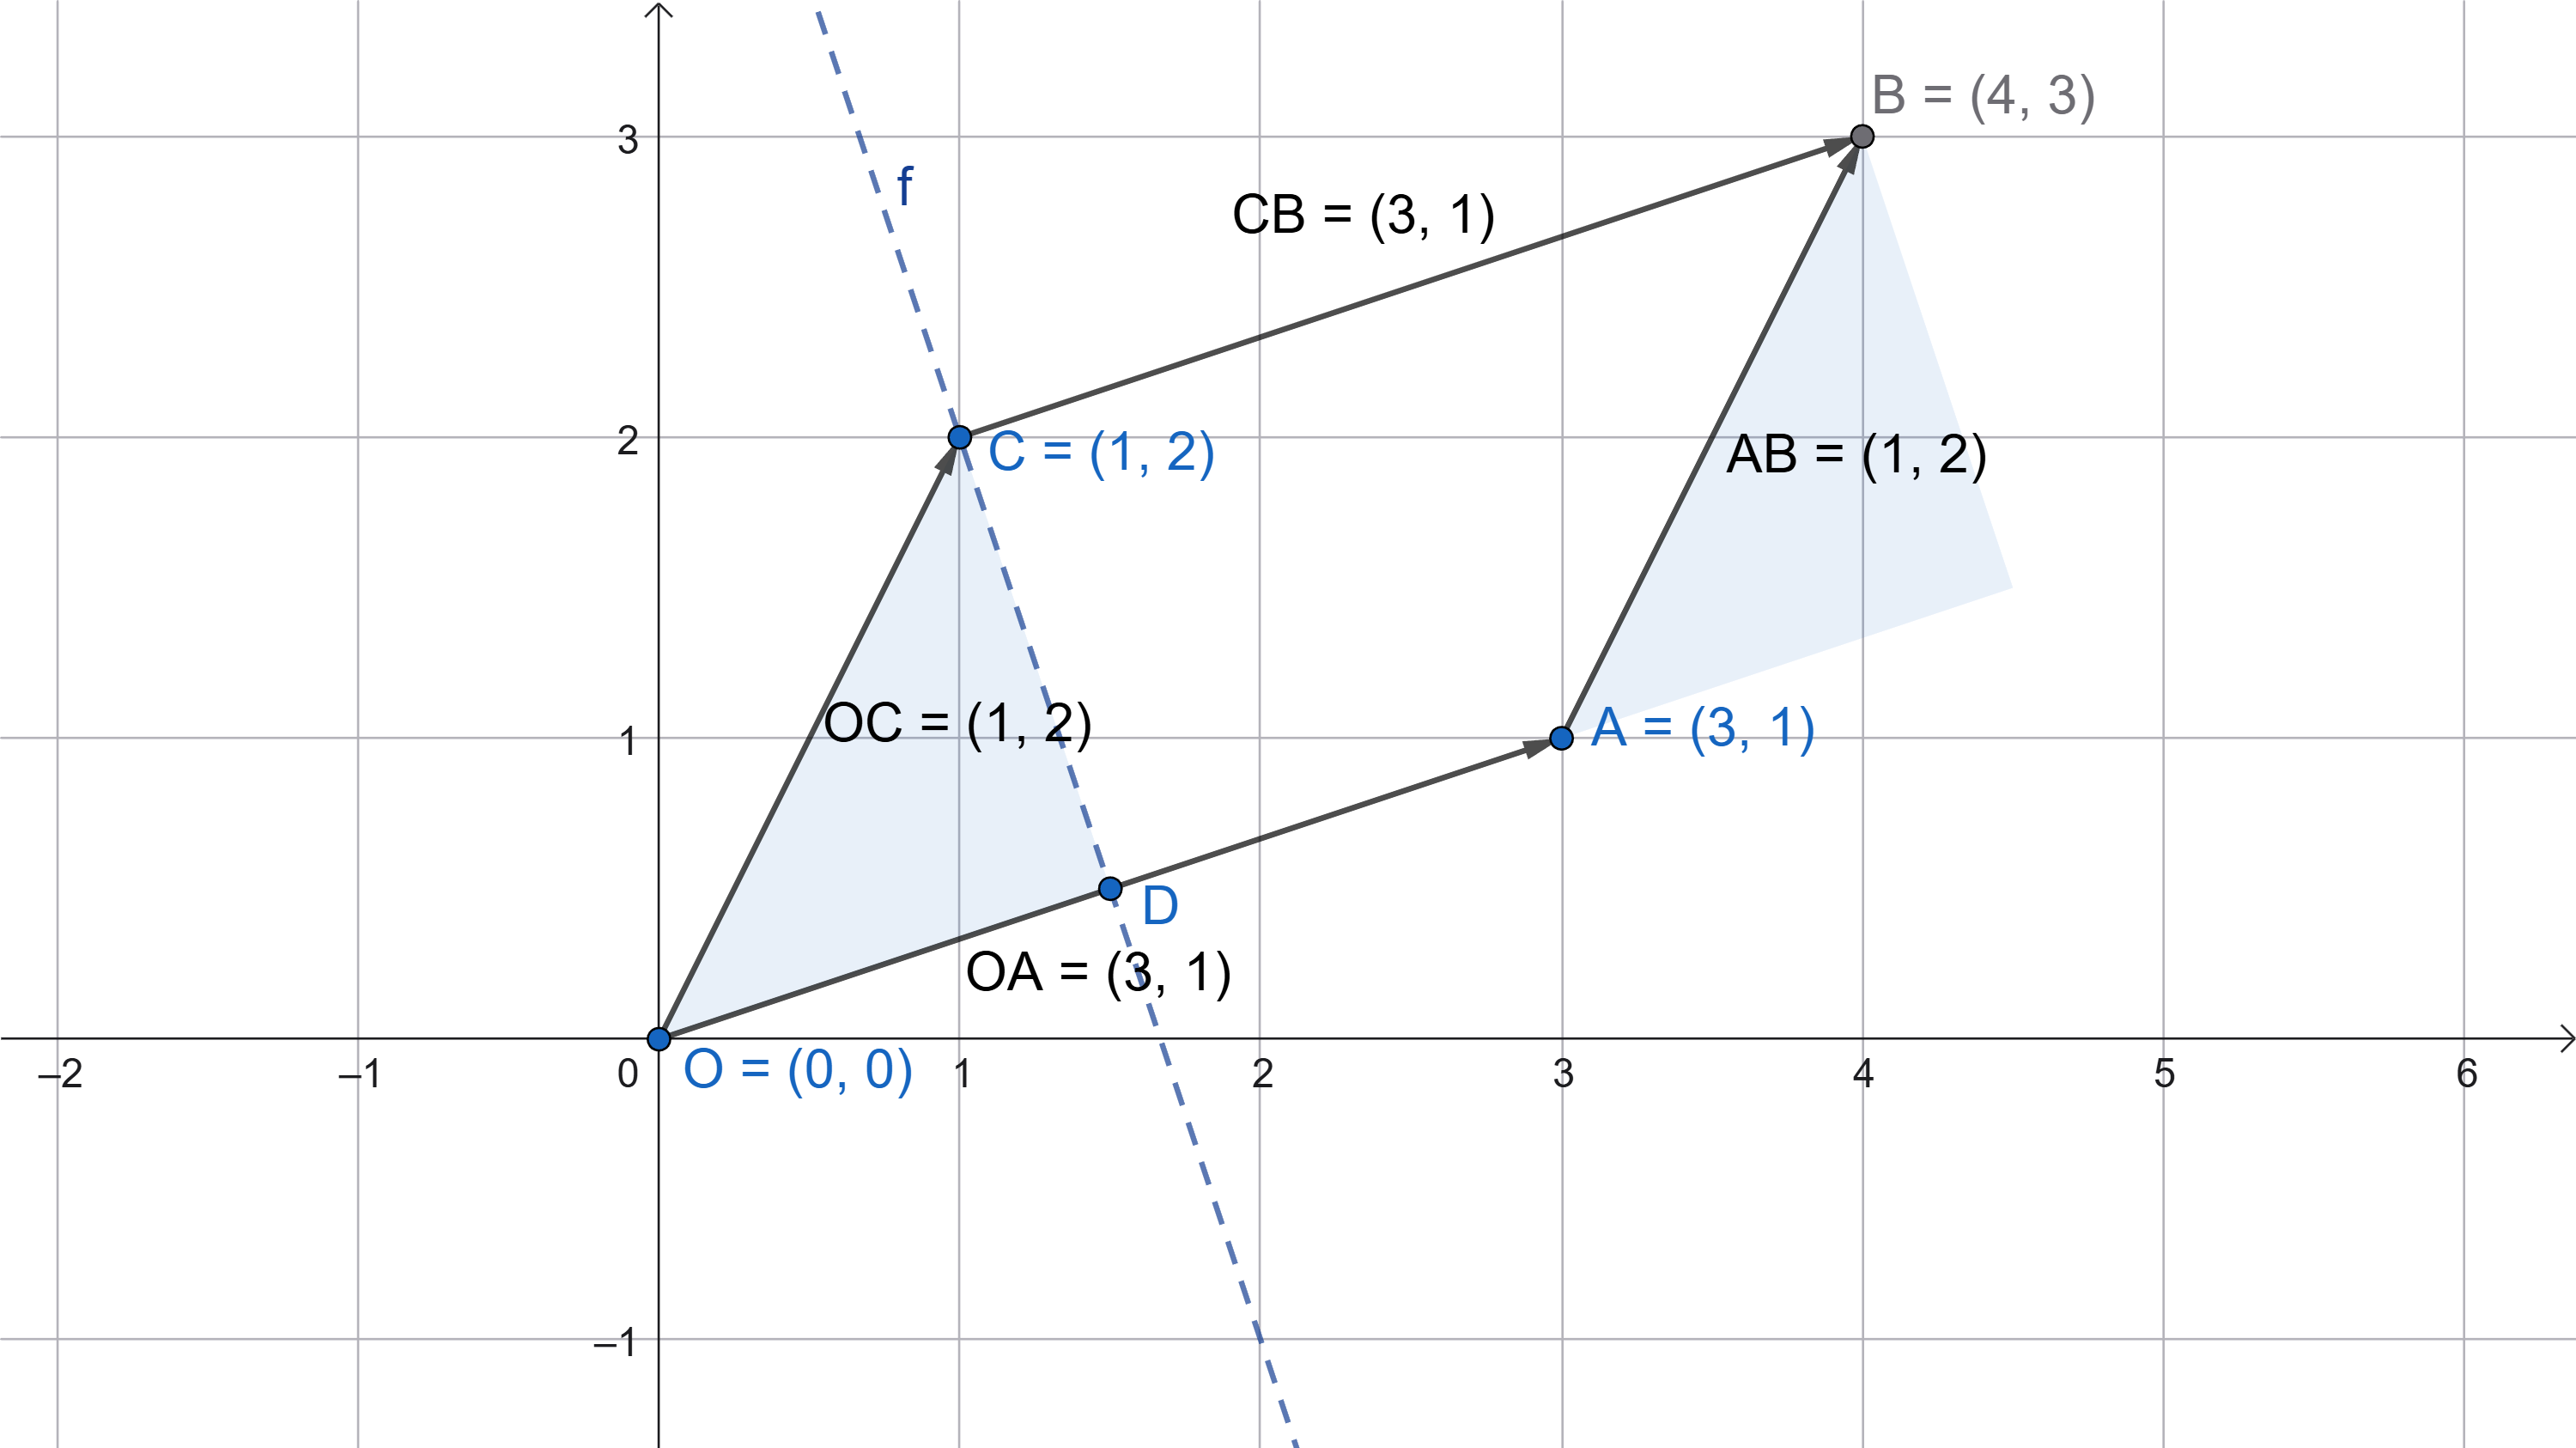
\includegraphics[width=0.7\textwidth]{Rectes al pla - 20 AF paral·lelogram àrea_4.png}
    \caption{Com convertir un paral·lelogram en un rectangle a efecte de càlculs d'àrea.}
\end{figure}

Per fer-ho, necessitem trobar la longitud de l'altura $h$, que és la distància entre el punt $C$ i la recta que conté la base ($OA$). Seguirem aquests passos:
\begin{enumerate}
    \item Trobar la recta base ($OA$).
    \item Trobar la recta perpendicular a la base que passa per $C$.
    \item Trobar el punt d'intersecció $D$ (peu de l'altura).
    \item Calcular la distància $CD$ i multiplicar-la per la base $|\vec{OA}|$.
\end{enumerate}

\subsubsection*{Pas A: Equació de la recta base (OA)}
El vector director és $\vec{OA} = (3, 1)$. El pendent és $m = 1/3$. Passa per $(0,0)$.
\[ y = \frac{1}{3}x \Rightarrow 3y = x \Rightarrow \boxed{x - 3y = 0} \]

\subsubsection*{Pas B: Equació de la recta perpendicular (altura)}
El vector director d'aquesta recta ha de ser perpendicular a $\vec{OA}$. El vector normal de la recta base $(1, -3)$ ens serveix com a vector director de l'altura, o simplement usem que el vector normal de l'altura serà el $\vec{OA} = (3, 1)$.
\[ 3x + 1y + K = 0 \]
Imposem que passi per $C(1, 2)$:
\[ 3(1) + 2 + K = 0 \Rightarrow 5 + K = 0 \Rightarrow K = -5 \]
Equació de l'altura: $\boxed{3x + y - 5 = 0}$

\begin{figure}[H]
    \centering
    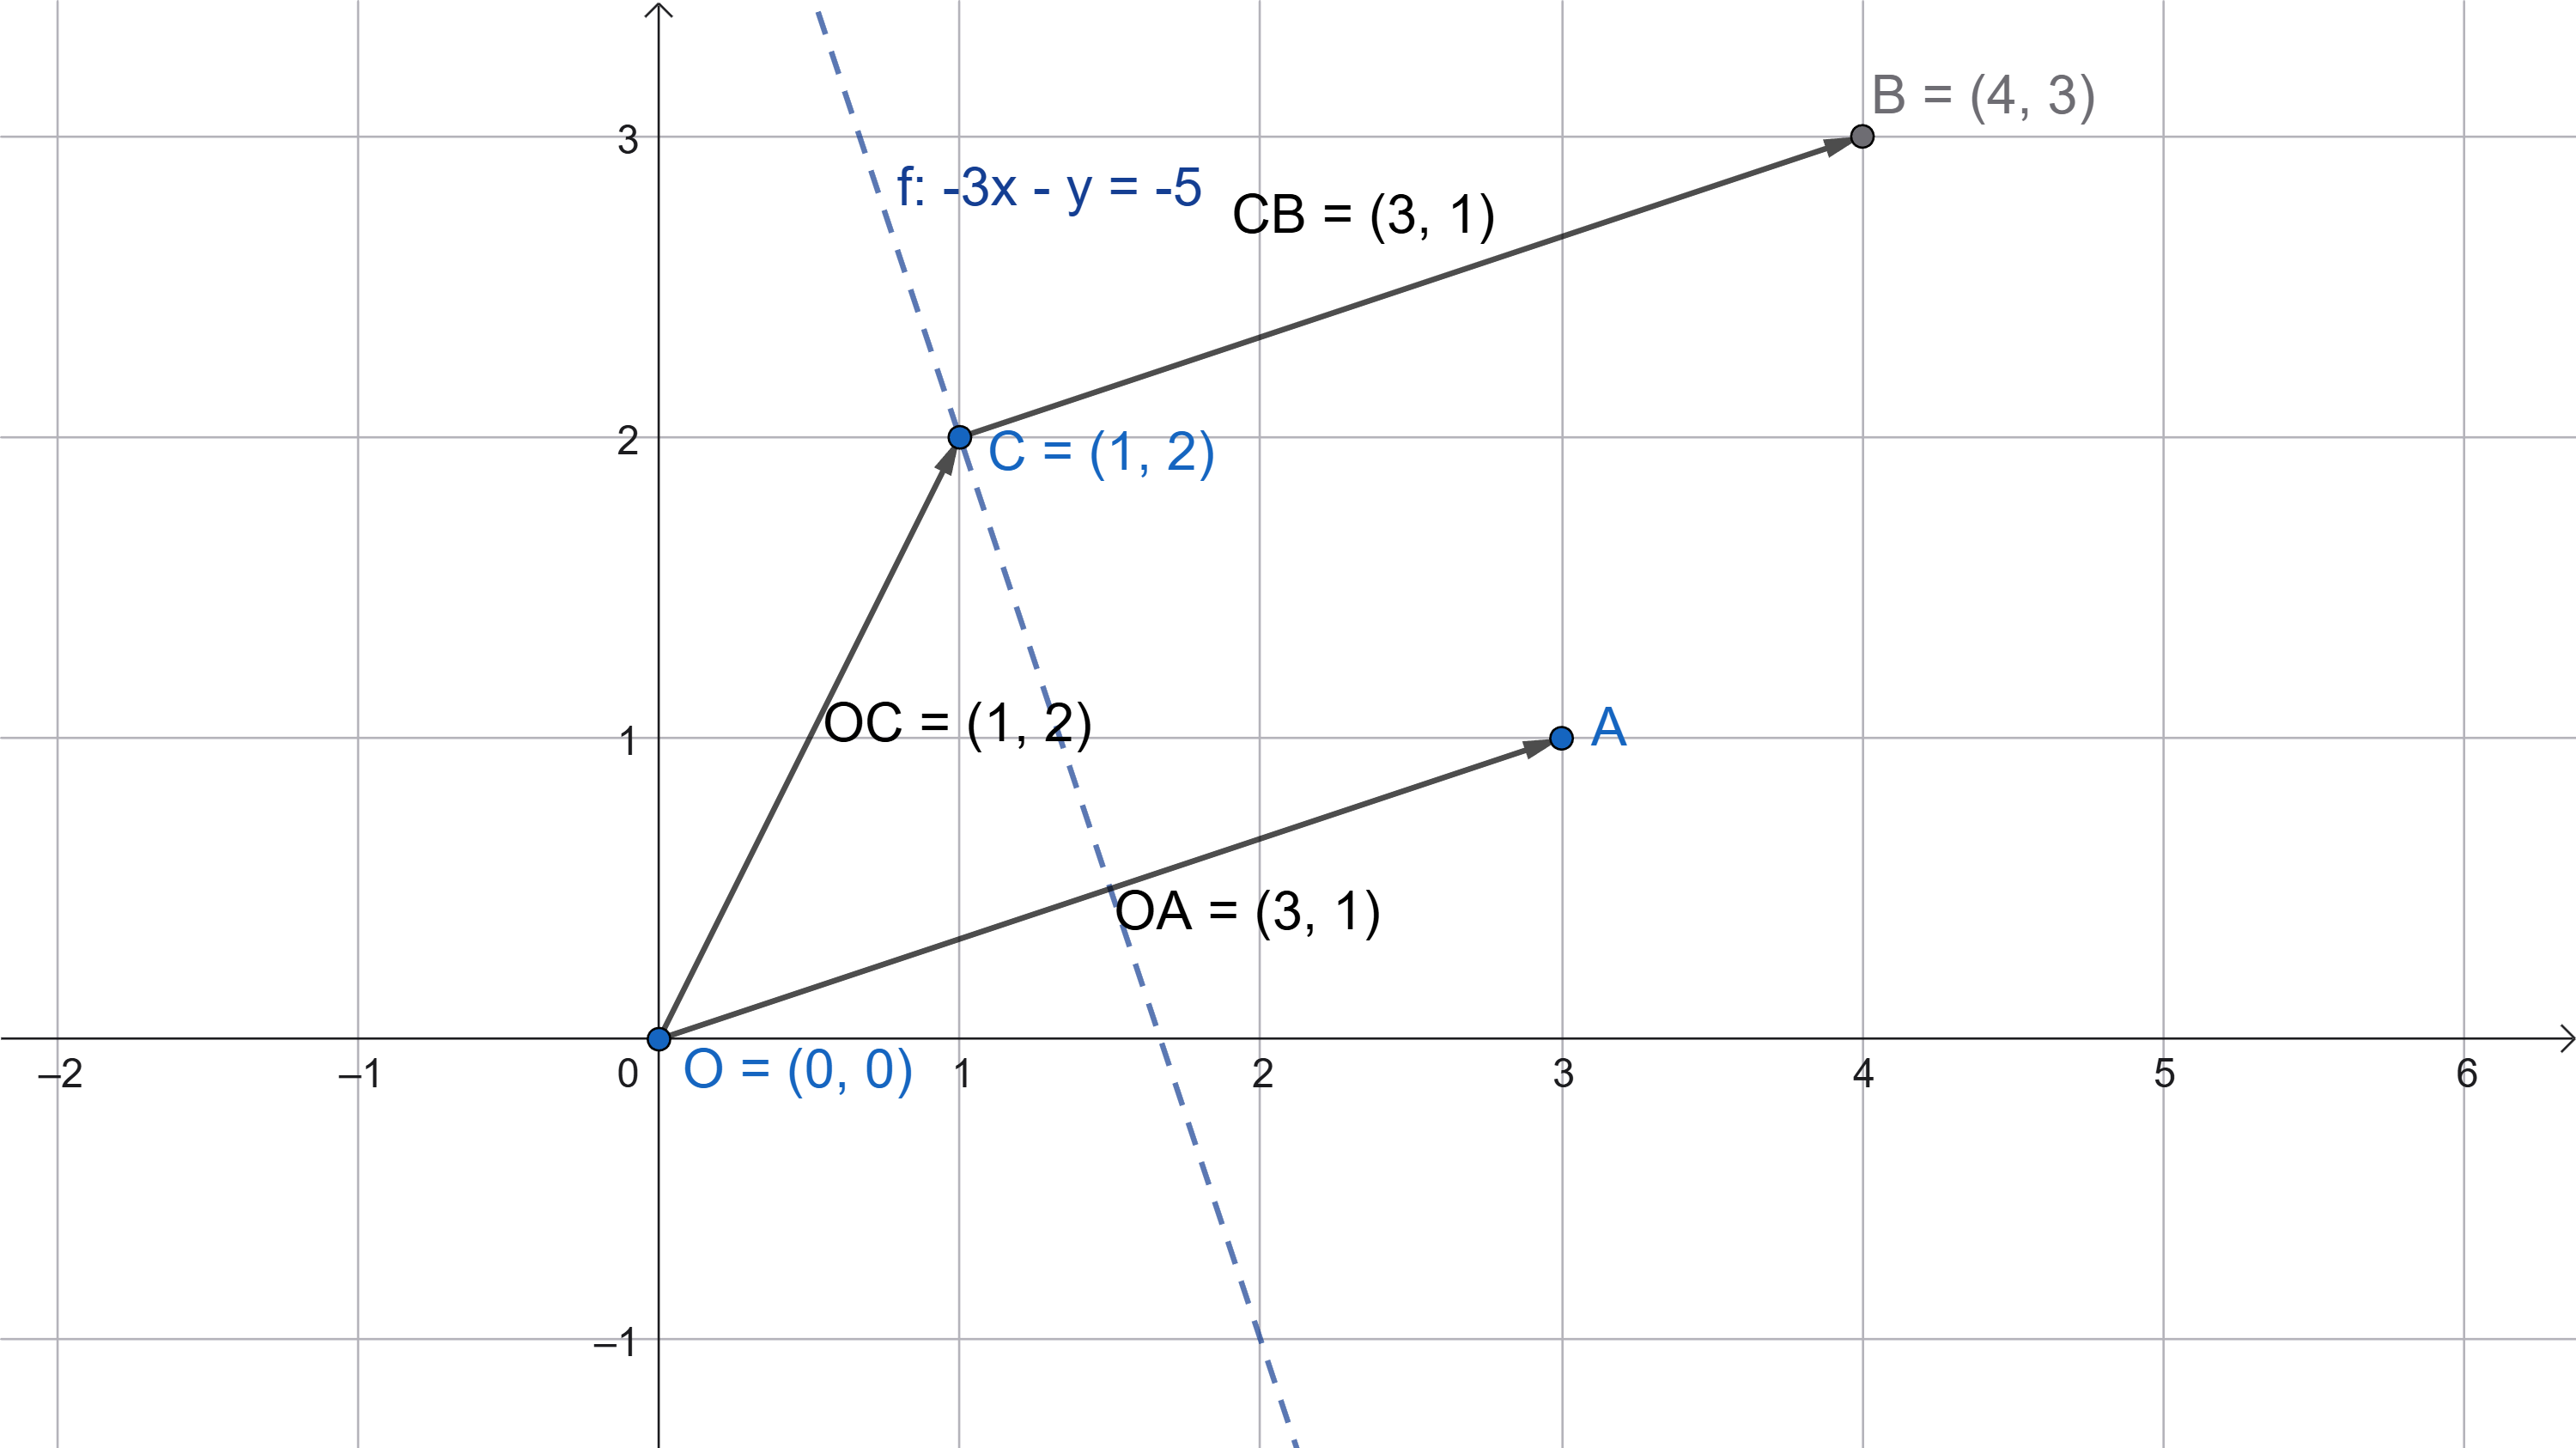
\includegraphics[width=0.7\textwidth]{Rectes al pla - 20 AF paral·lelogram àrea_5.png}
    \caption{Recta perpendicular a la base traçada des de C.}
\end{figure}

\subsubsection*{Pas C: Punt d'intersecció D}
Resolem el sistema format per la recta base i l'altura per trobar el punt $D$:
\[
\begin{cases}
x - 3y = 0 \Rightarrow x = 3y \\
3x + y - 5 = 0
\end{cases}
\]
Substituïm la primera en la segona:
\[ 3(3y) + y - 5 = 0 \Rightarrow 9y + y = 5 \Rightarrow 10y = 5 \Rightarrow y = 0,5 \]
Trobem la x:
\[ x = 3(0,5) = 1,5 \]
El punt d'intersecció és $\boxed{D(1.5, 0.5)}$.

\begin{figure}[H]
    \centering
    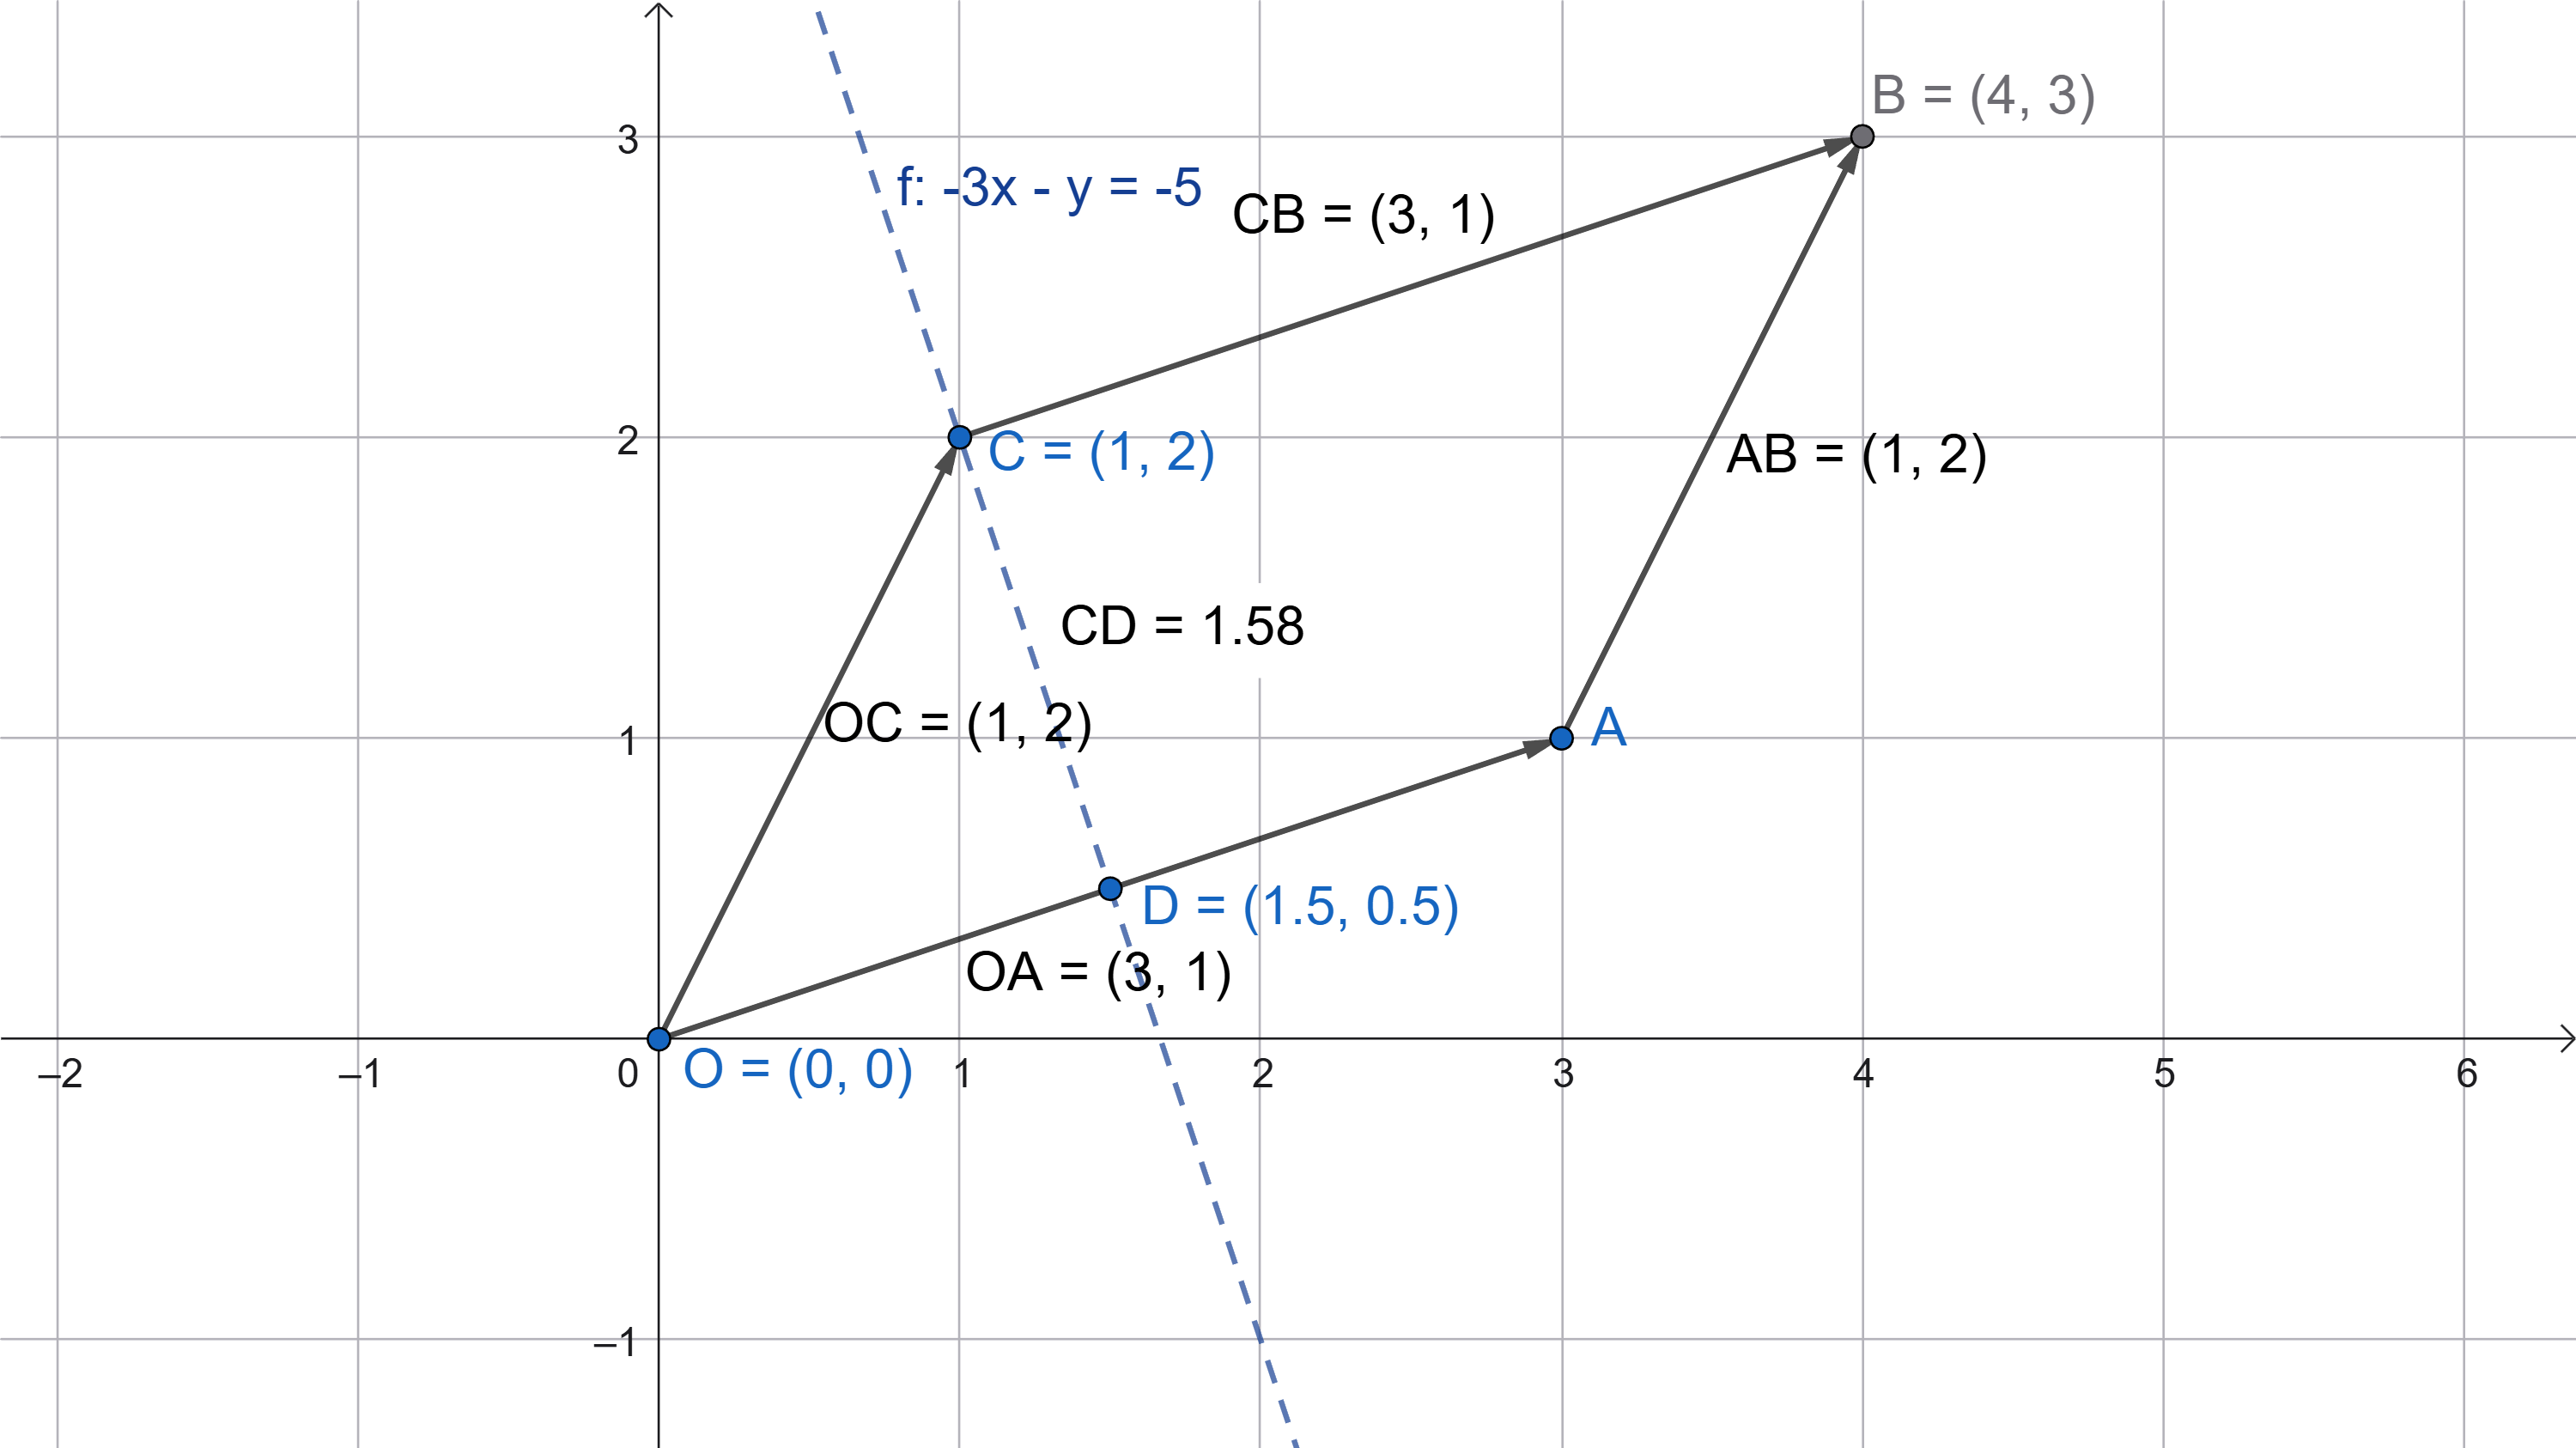
\includegraphics[width=0.7\textwidth]{Rectes al pla - 20 AF paral·lelogram àrea_8.png}
    \caption{El segment CD és l'altura del paral·lelogram.}
\end{figure}

\subsubsection*{Pas D: Càlcul final de l'àrea}

\begin{itemize}
    \item \textbf{Base ($|\vec{OA}|$):}
    \[ |\vec{OA}| = \sqrt{3^2 + 1^2} = \sqrt{9+1} = \sqrt{10} \approx 3,16 \, u \]
    
    \item \textbf{Altura ($|\vec{CD}|$):}
    \[ \vec{CD} = D - C = (1.5, 0.5) - (1, 2) = (0.5, -1.5) \]
    \[ |\vec{CD}| = \sqrt{0,5^2 + (-1,5)^2} = \sqrt{0,25 + 2,25} = \sqrt{2,5} \approx 1,58 \, u \]
\end{itemize}

Finalment, fem el producte:
\[ \text{Àrea} = \sqrt{10} \cdot \sqrt{2,5} = \sqrt{25} = \boxed{5 \, u^2} \]

% --- EXERCICI 21 ---
\section*{Exercici 21 Activitats Finals}
\textbf{Determina l'equació de les rectes que contenen les altures del triangle de vèrtexs $A(-2, 1)$, $B(0, 2)$ i $C(4, 0)$.}

\vspace{0.5cm}

\textbf{Definició prèvia:} Una altura és una recta que passa per un vèrtex del triangle i és perpendicular al costat oposat. Per tant, el vector del costat oposat actuarà com a \textbf{vector normal} ($\vec{n}$) de la recta de l'altura.

Comencem representant els tres vèrtexs al pla:

\begin{figure}[H]
    \centering
    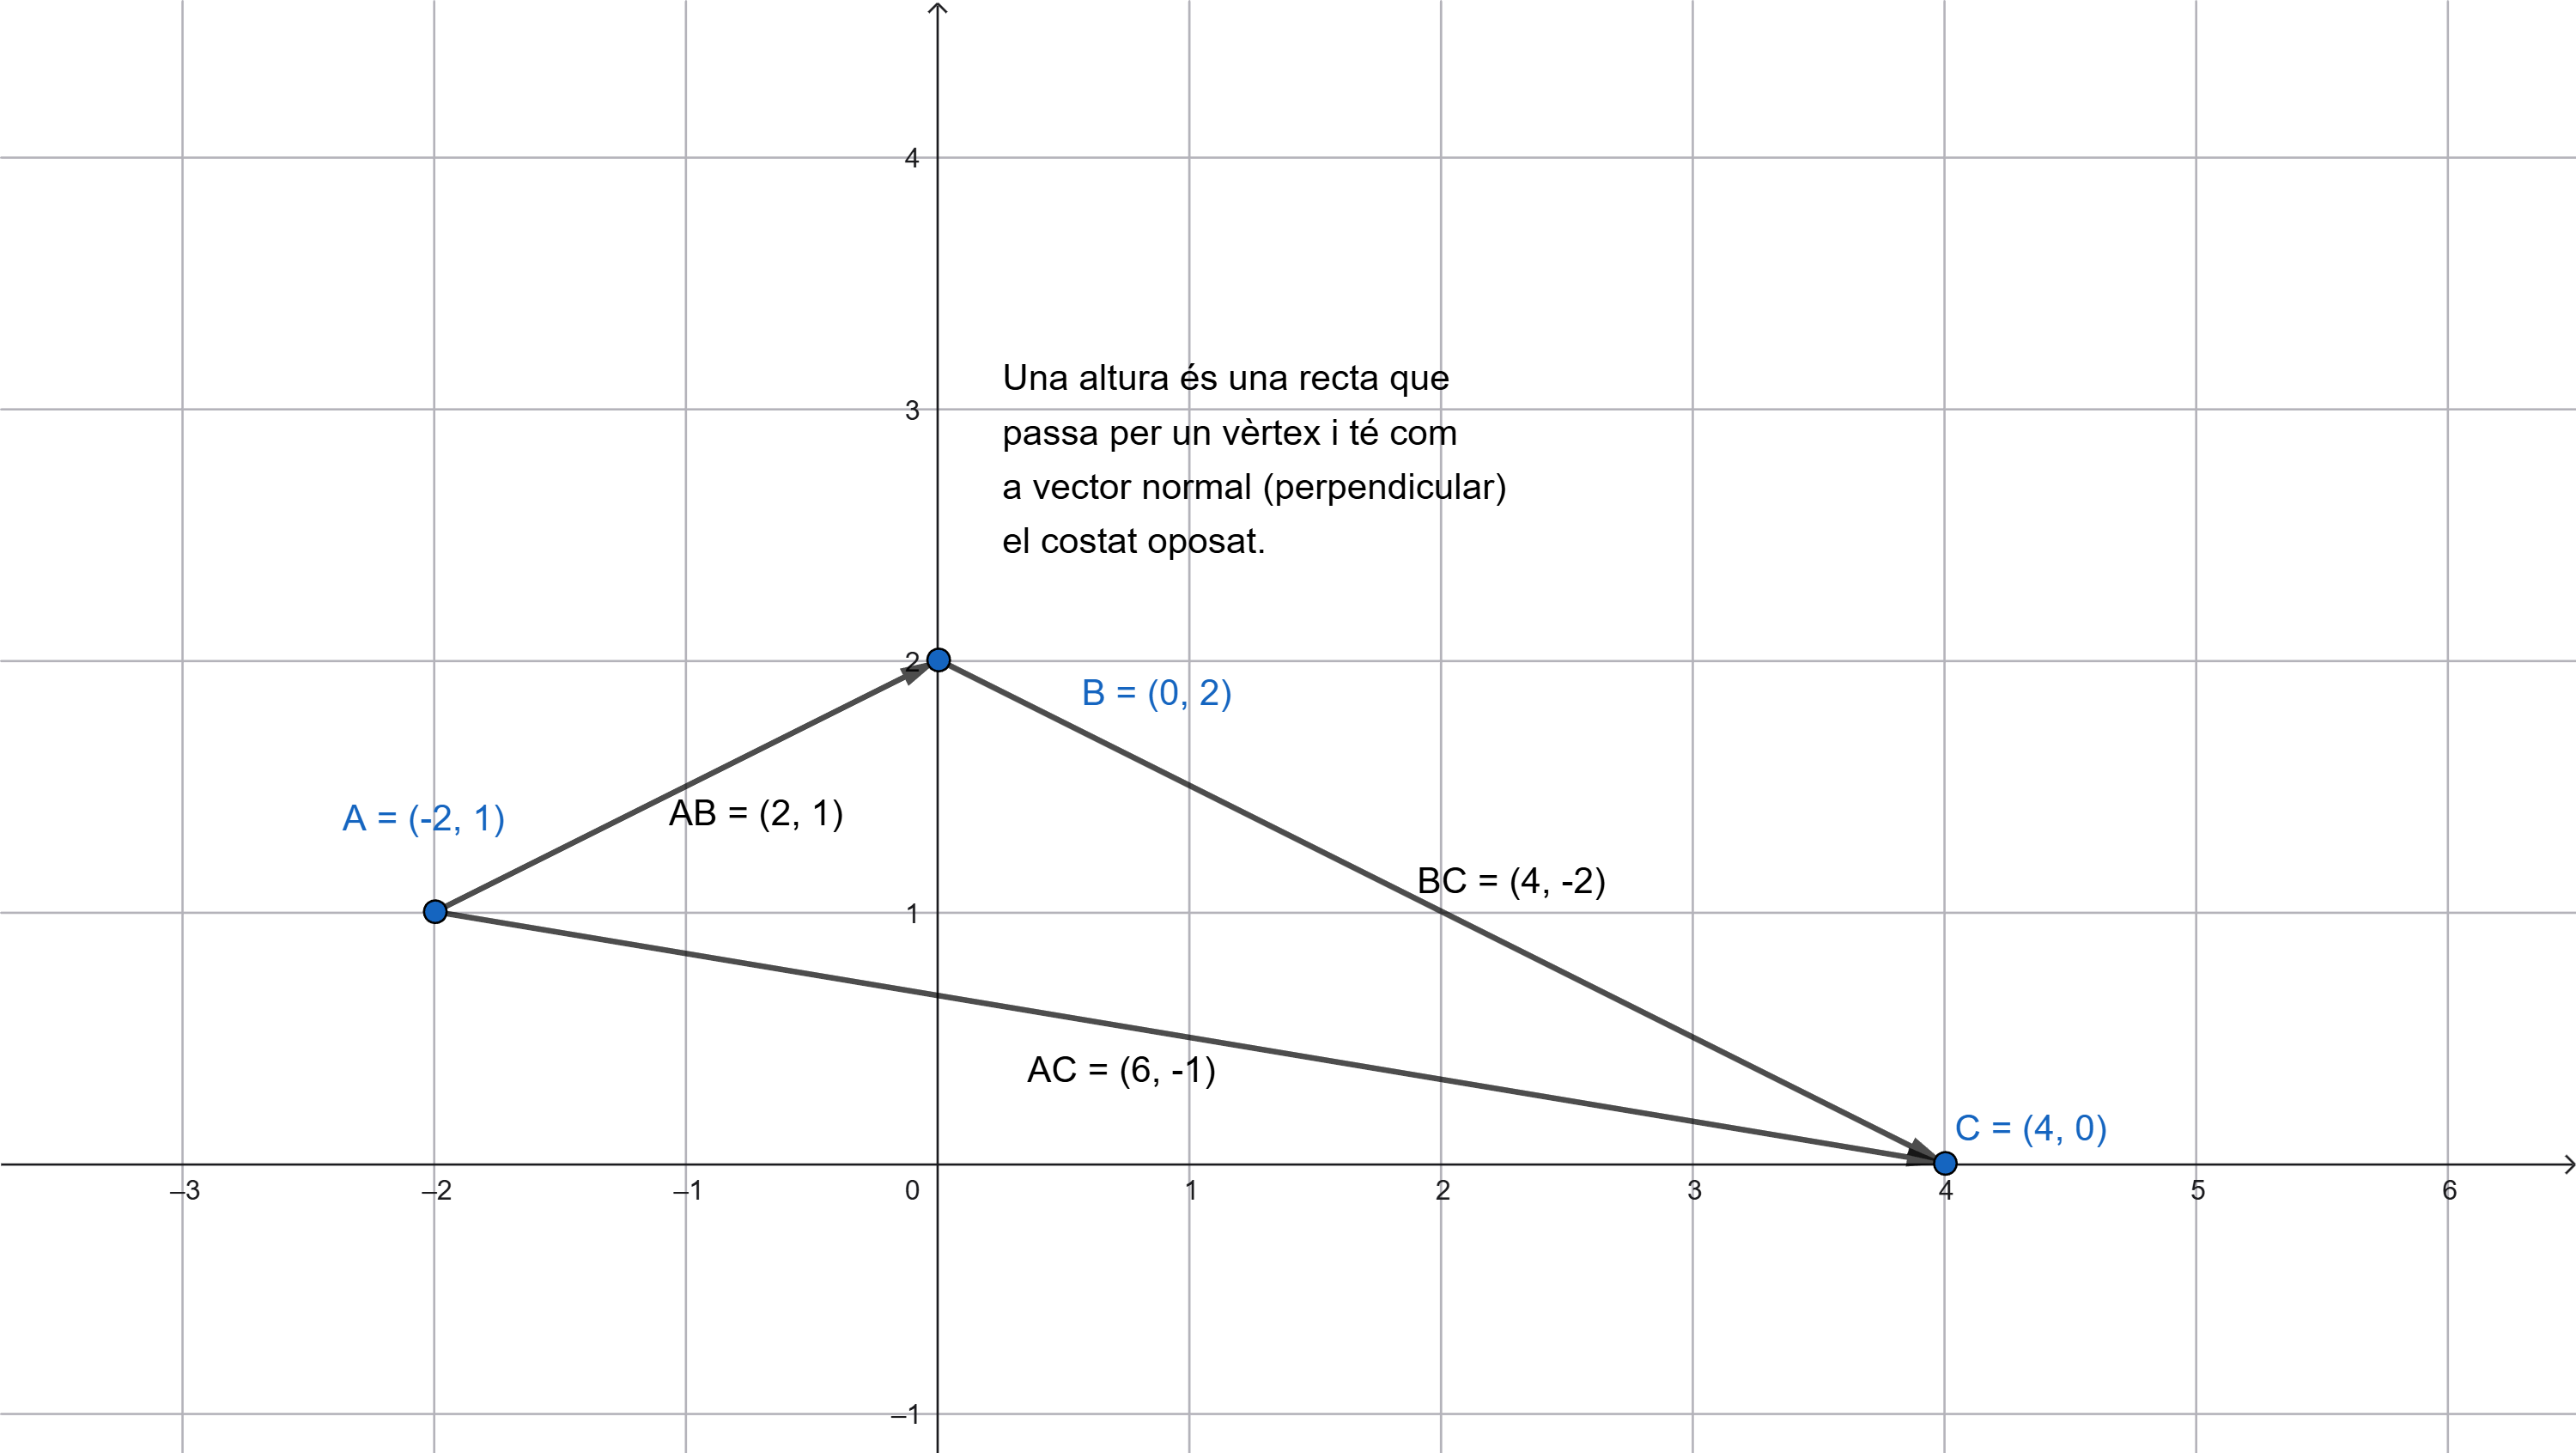
\includegraphics[width=0.7\textwidth]{Rectes - Altures triangle 21 AF_1.png}
    \caption{Representació inicial del triangle $ABC$.}
\end{figure}

\newpage

% --- Altura h_A ---
\subsection*{1. Altura sobre el vèrtex A ($h_A$)}

L'altura $h_A$ passa pel punt $A(-2, 1)$ i és perpendicular al costat $BC$.
\begin{enumerate}
    \item \textbf{Calculem el vector director del costat oposat ($\vec{BC}$):}
    \[ \vec{BC} = C - B = (4, 0) - (0, 2) = (4, -2) \]
    Podem simplificar aquest vector per treballar amb nombres més petits (ja que la direcció és la mateixa): $\vec{v} = (2, -1)$.
    
    \item \textbf{Identifiquem el vector normal:}
    Com que $h_A \perp BC$, el vector $\vec{BC}$ és el vector normal ($\vec{n}$) de l'altura $h_A$.
    \[ \vec{n}_{h_A} = (4, -2) \quad \text{o simplificat} \quad (2, -1) \]
    
    \begin{figure}[H]
        \centering
        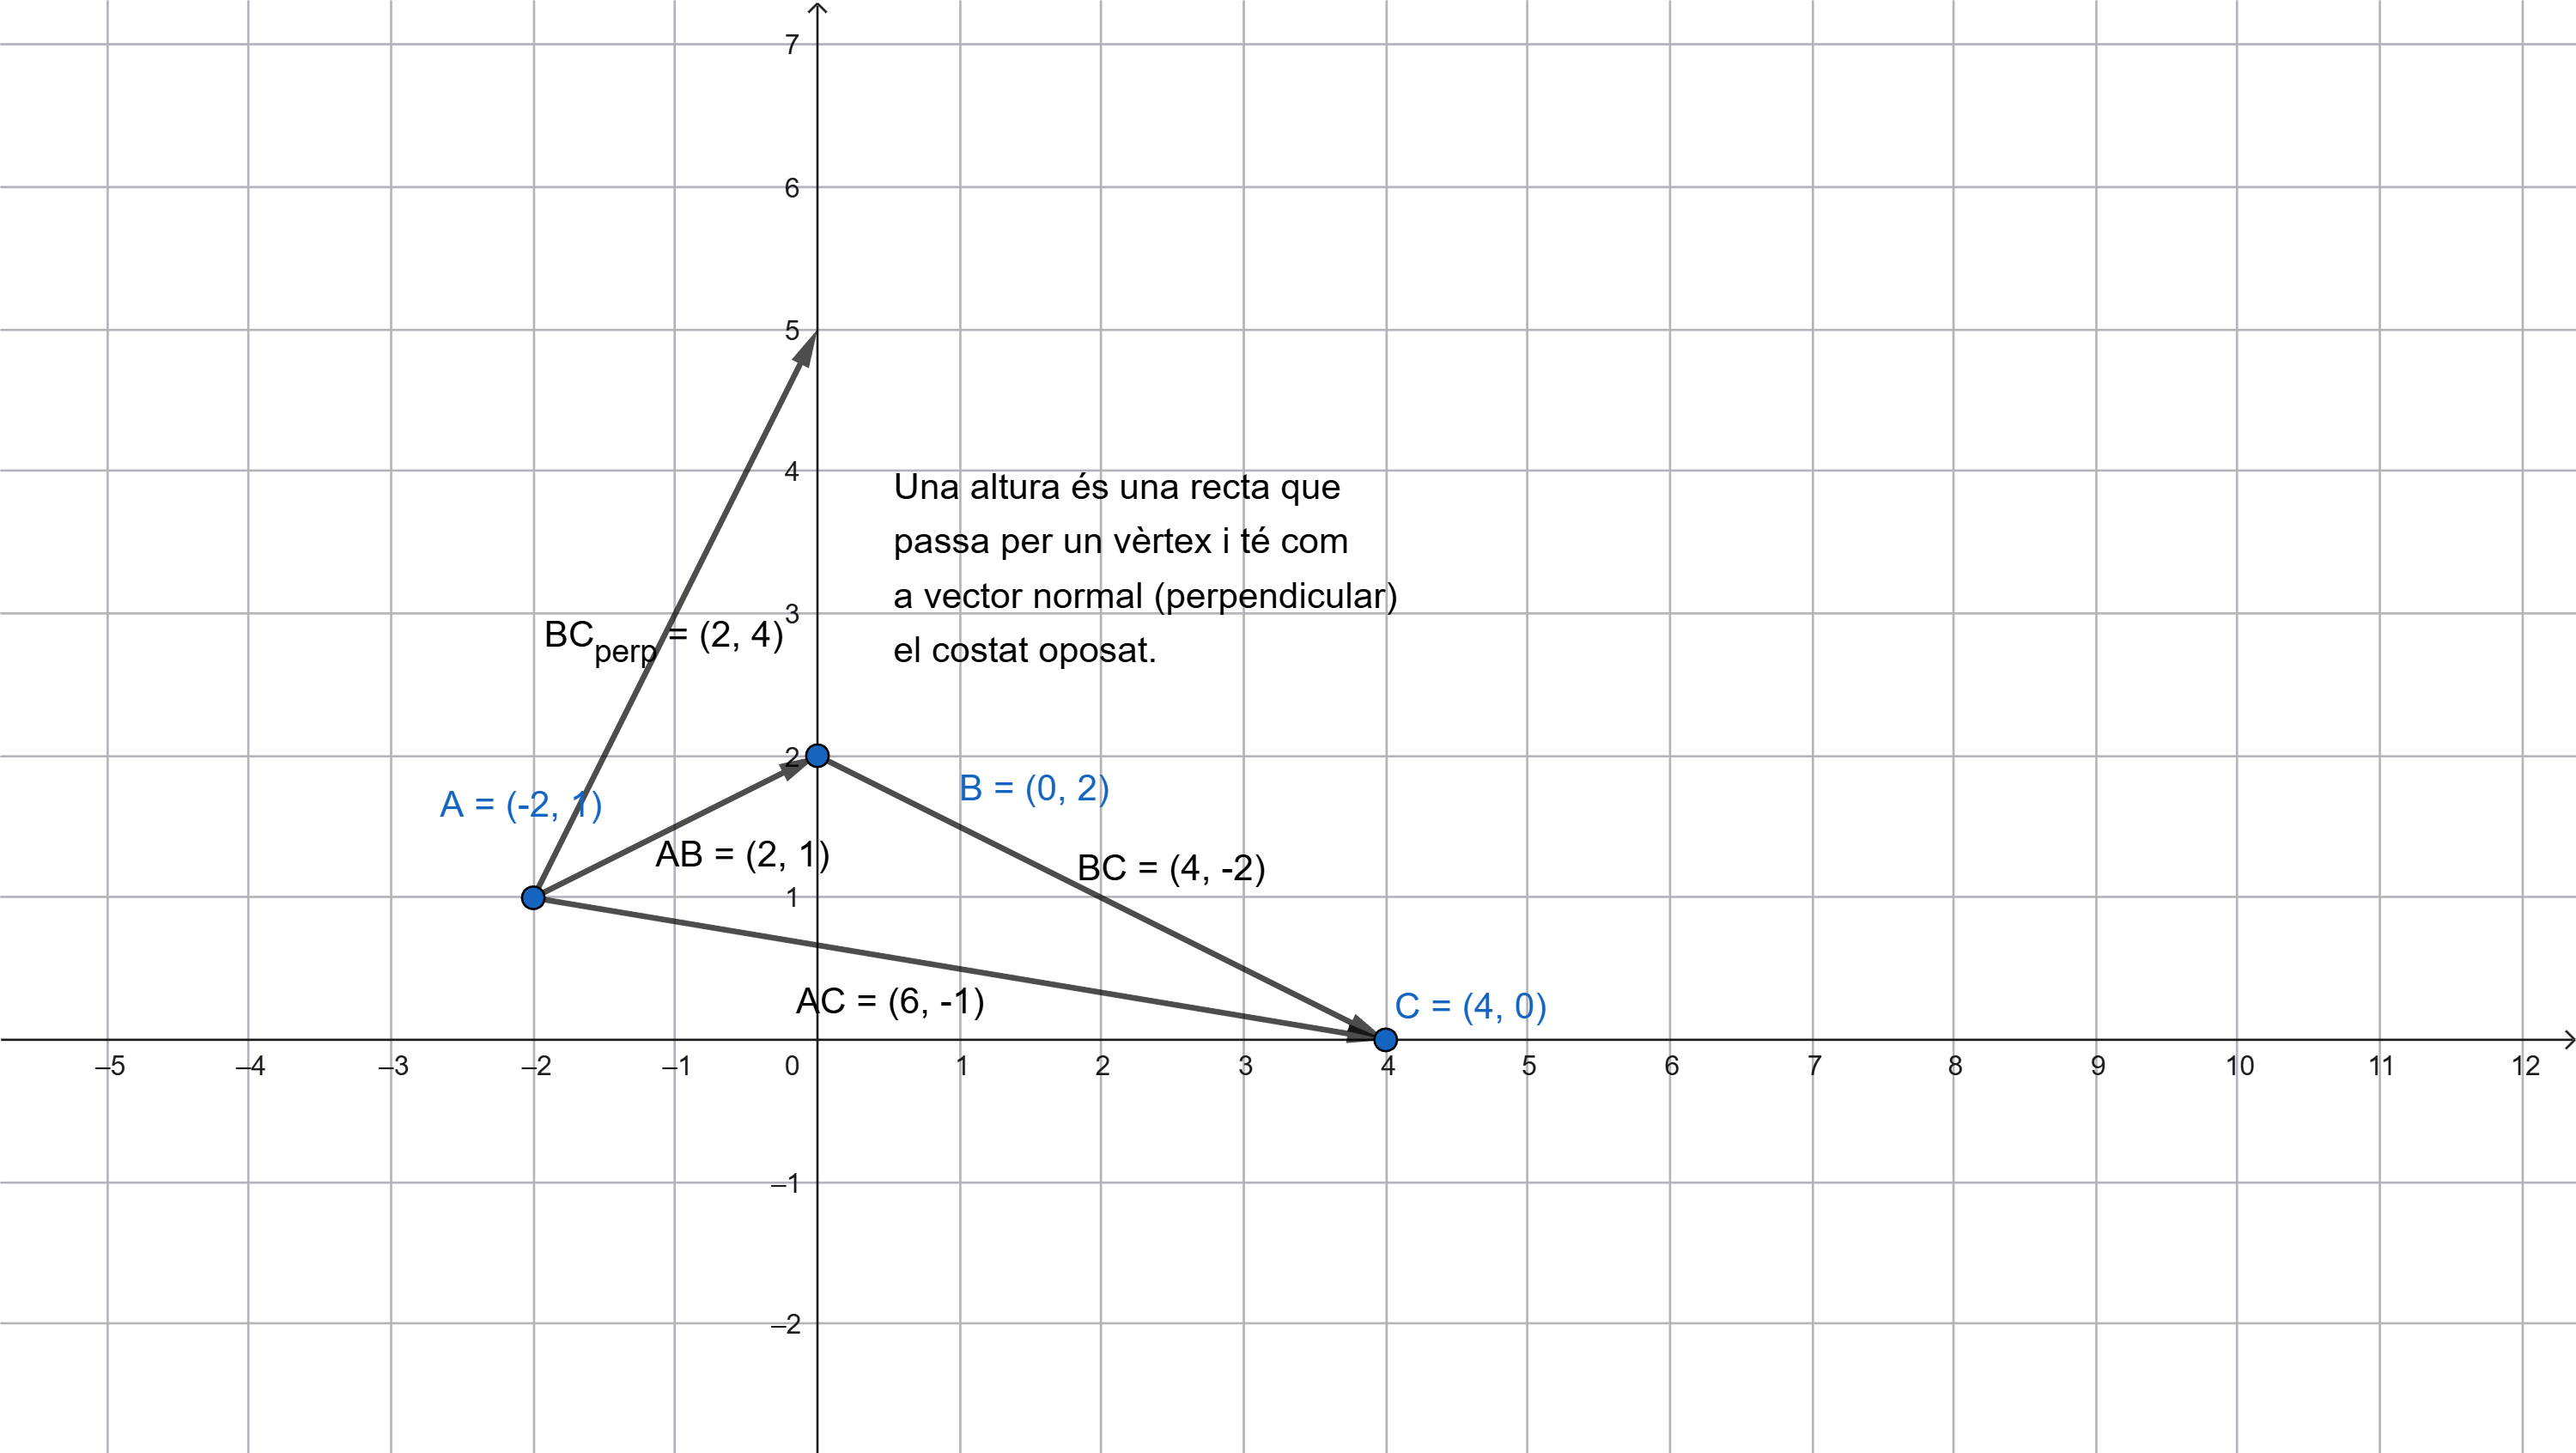
\includegraphics[width=0.7\textwidth]{Rectes - Altures triangle 21 AF_2.png}
        \caption{El vector $\vec{BC}$ actua com a vector normal per a l'altura que passa per $A$.}
    \end{figure}

    \item \textbf{Trobem l'equació general:}
    L'equació general té la forma $Ax + By + C = 0$, on $(A, B)$ és el vector normal. Usant $\vec{n} = (2, -1)$:
    \[ 2x - 1y + C = 0 \]
    
    Ara imposem que la recta passi pel punt $A(-2, 1)$. Substituïm $x$ i $y$:
    \[ 2(-2) - (1) + C = 0 \]
    \[ -4 - 1 + C = 0 \Rightarrow -5 + C = 0 \Rightarrow C = 5 \]
    
    \textbf{L'equació de l'altura $h_A$ és:}
    \[ \boxed{2x - y + 5 = 0} \]
\end{enumerate}

\begin{figure}[H]
    \centering
    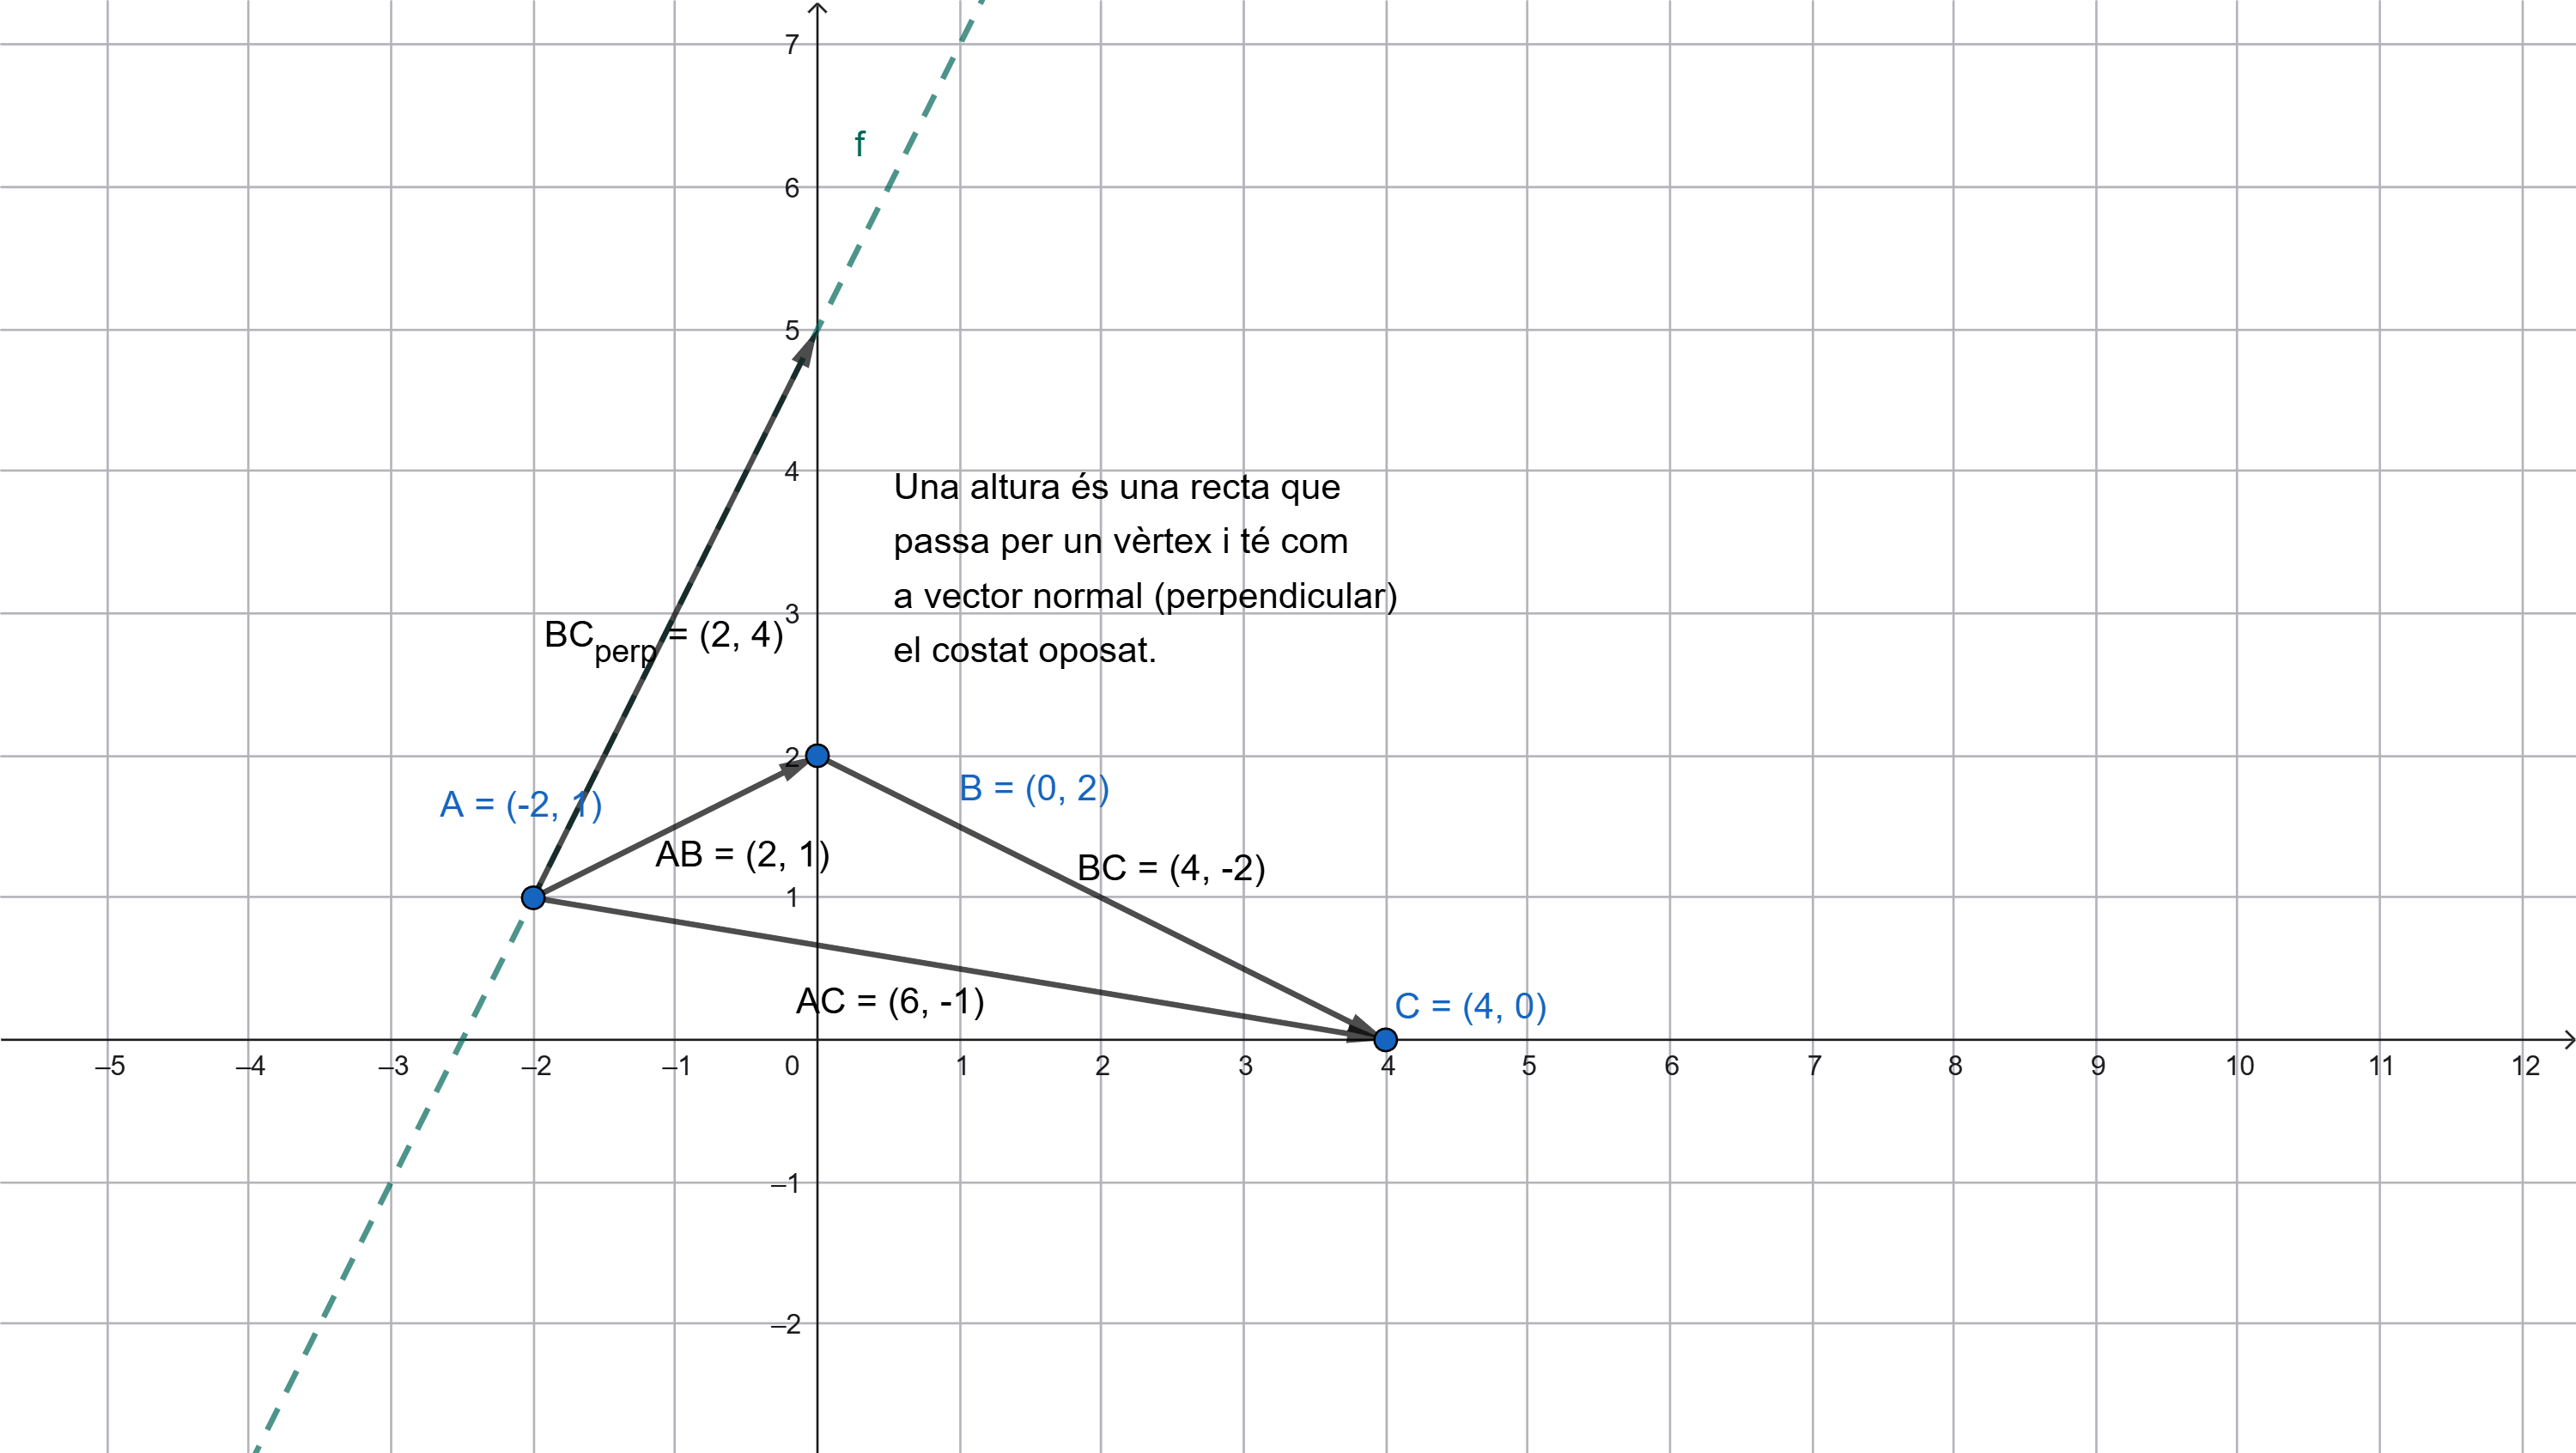
\includegraphics[width=0.7\textwidth]{Rectes - Altures triangle 21 AF_3.png}
    \caption{Representació de l'altura $h_A$.}
\end{figure}

\newpage

% --- Altura h_C ---
\subsection*{2. Altura sobre el vèrtex C ($h_C$)}

L'altura $h_C$ passa pel punt $C(4, 0)$ i és perpendicular al costat $AB$.

\begin{enumerate}
    \item \textbf{Calculem el vector director del costat oposat ($\vec{AB}$):}
    \[ \vec{AB} = B - A = (0, 2) - (-2, 1) = (2, 1) \]
    
    \item \textbf{Identifiquem el vector normal:}
    El vector $\vec{AB}$ és el vector normal ($\vec{n}$) de l'altura $h_C$.
    \[ \vec{n}_{h_C} = (2, 1) \]

    \begin{figure}[H]
        \centering
        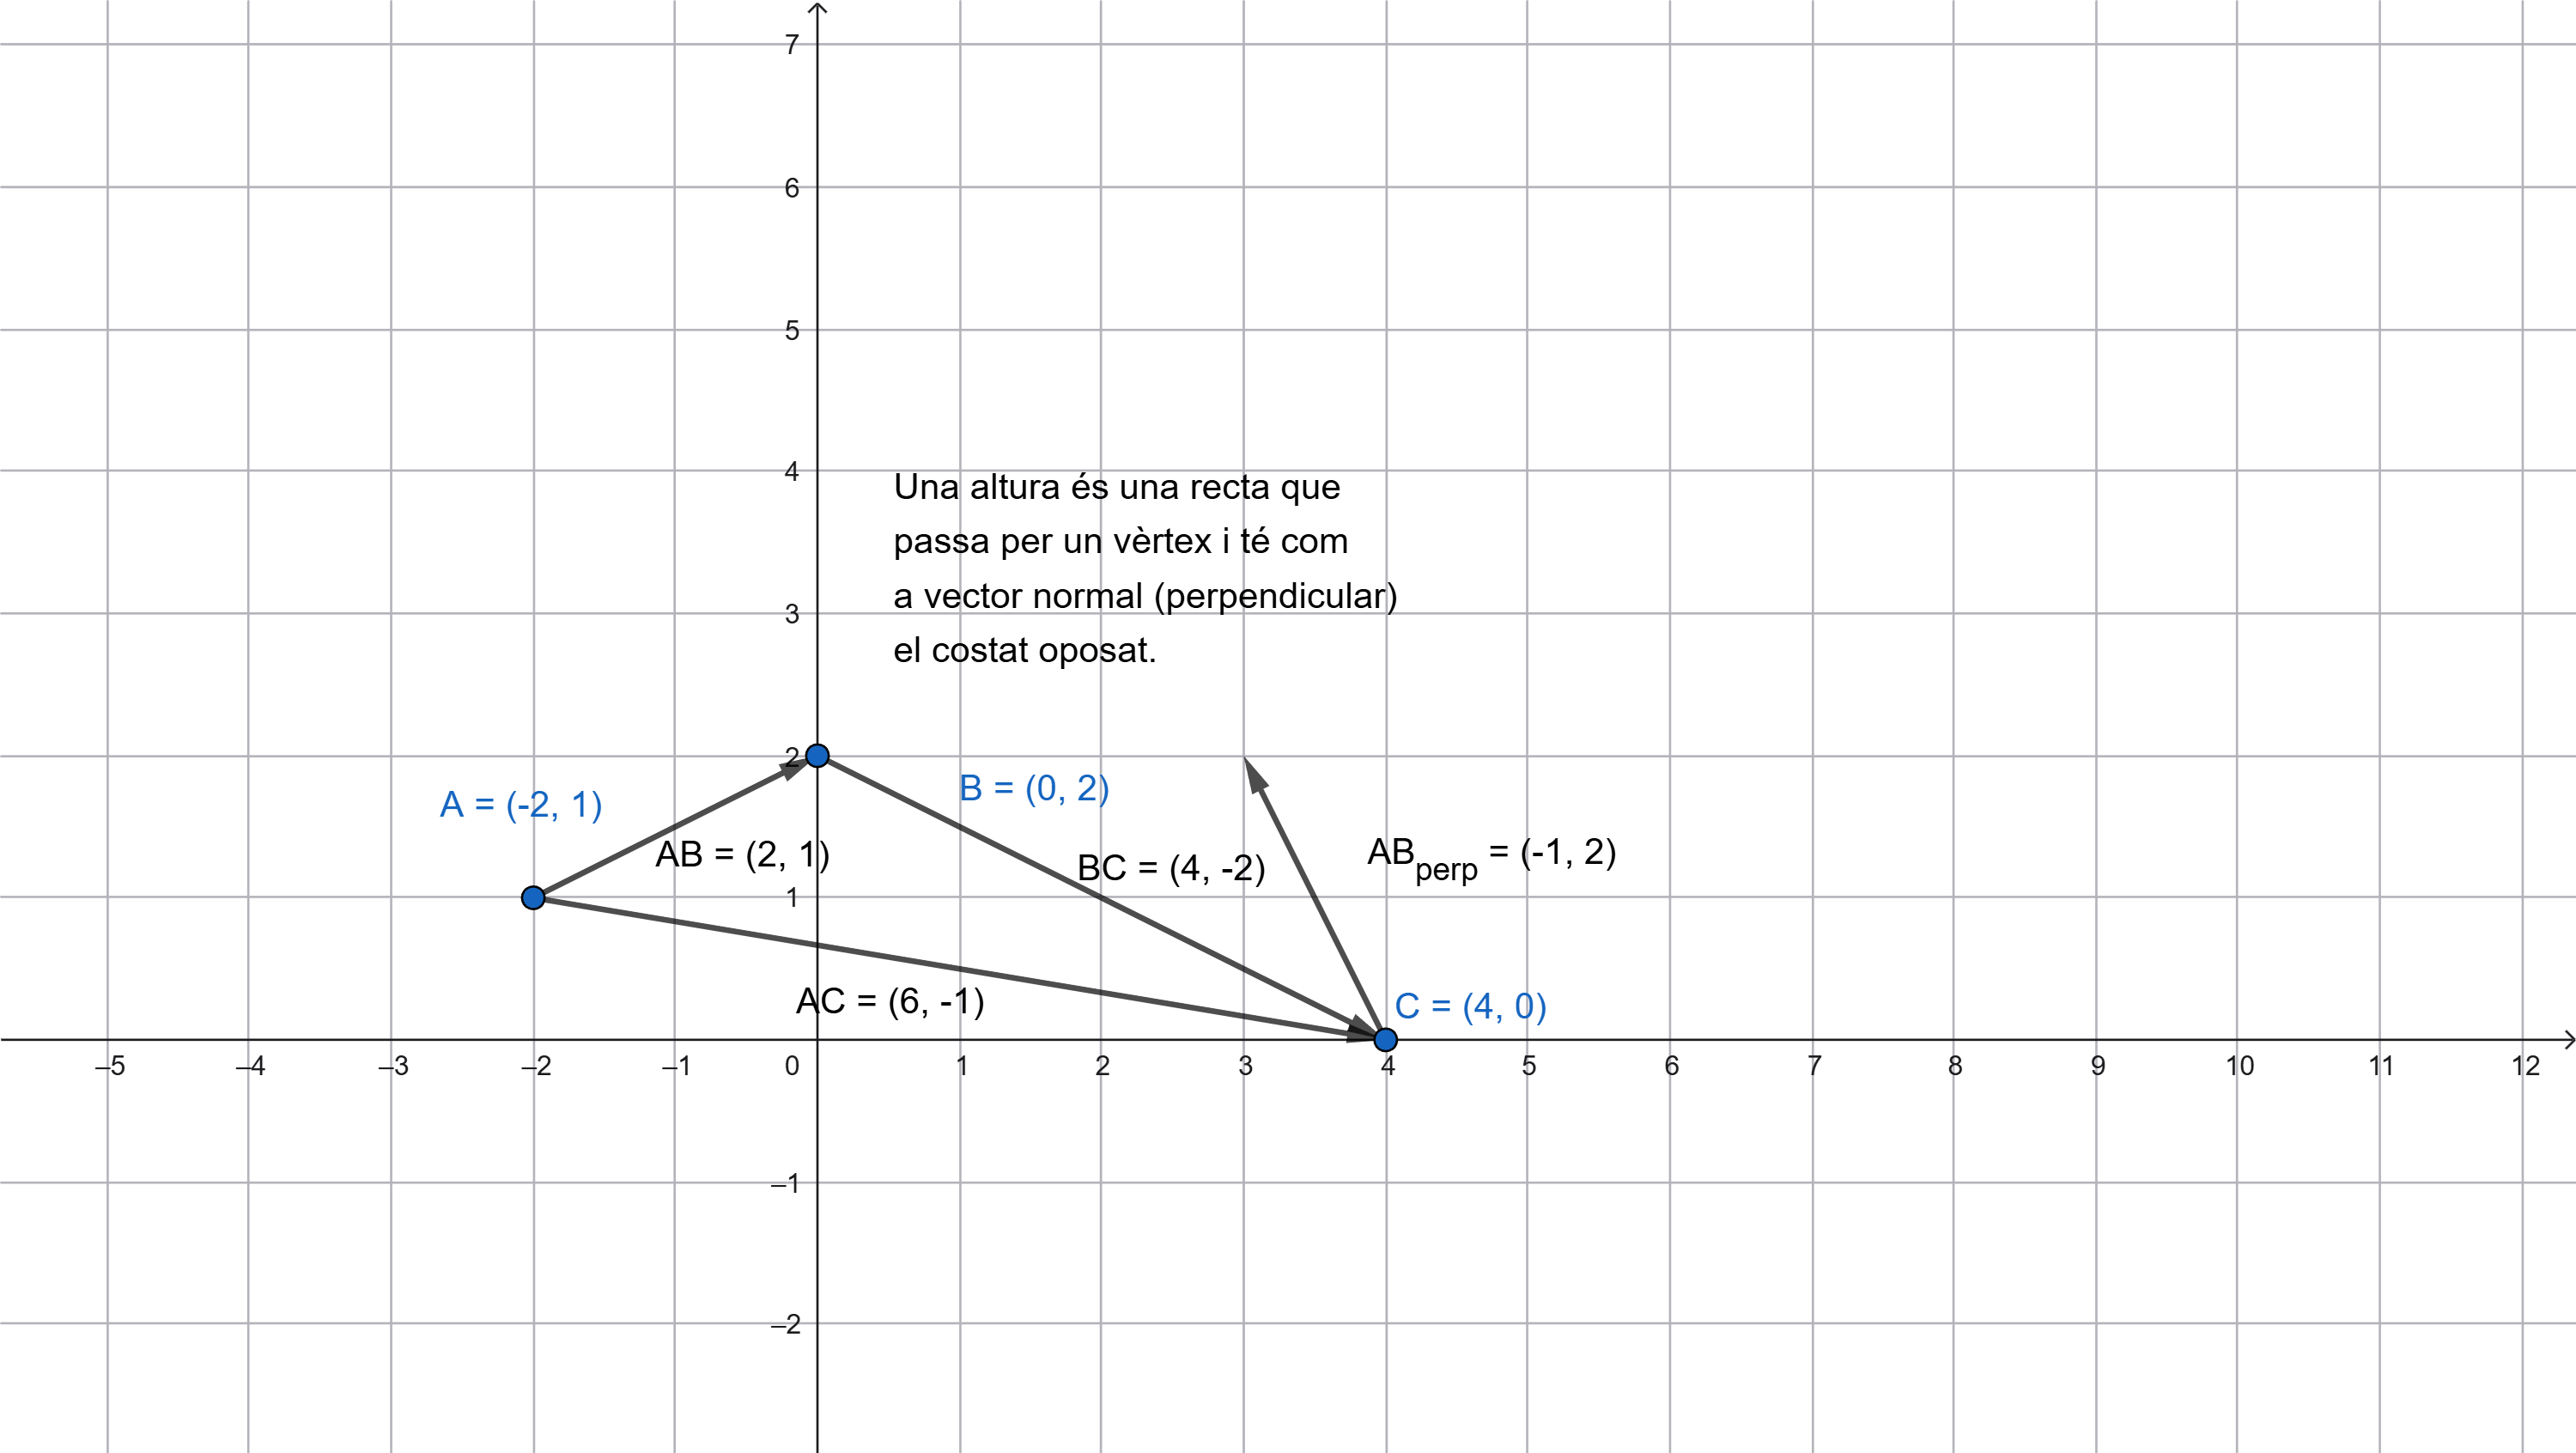
\includegraphics[width=0.7\textwidth]{Rectes - Altures triangle 21 AF_4.png}
        \caption{El vector $\vec{AB}$ defineix la direcció perpendicular per a $h_C$.}
    \end{figure}

    \item \textbf{Trobem l'equació general:}
    Usant el vector normal $(2, 1)$, l'equació és $2x + y + C = 0$.
    Imposem que passi pel vèrtex $C(4, 0)$:
    \[ 2(4) + 0 + C = 0 \]
    \[ 8 + C = 0 \Rightarrow C = -8 \]
    
    \textbf{L'equació de l'altura $h_C$ és:}
    \[ \boxed{2x + y - 8 = 0} \]
\end{enumerate}

\begin{figure}[H]
    \centering
    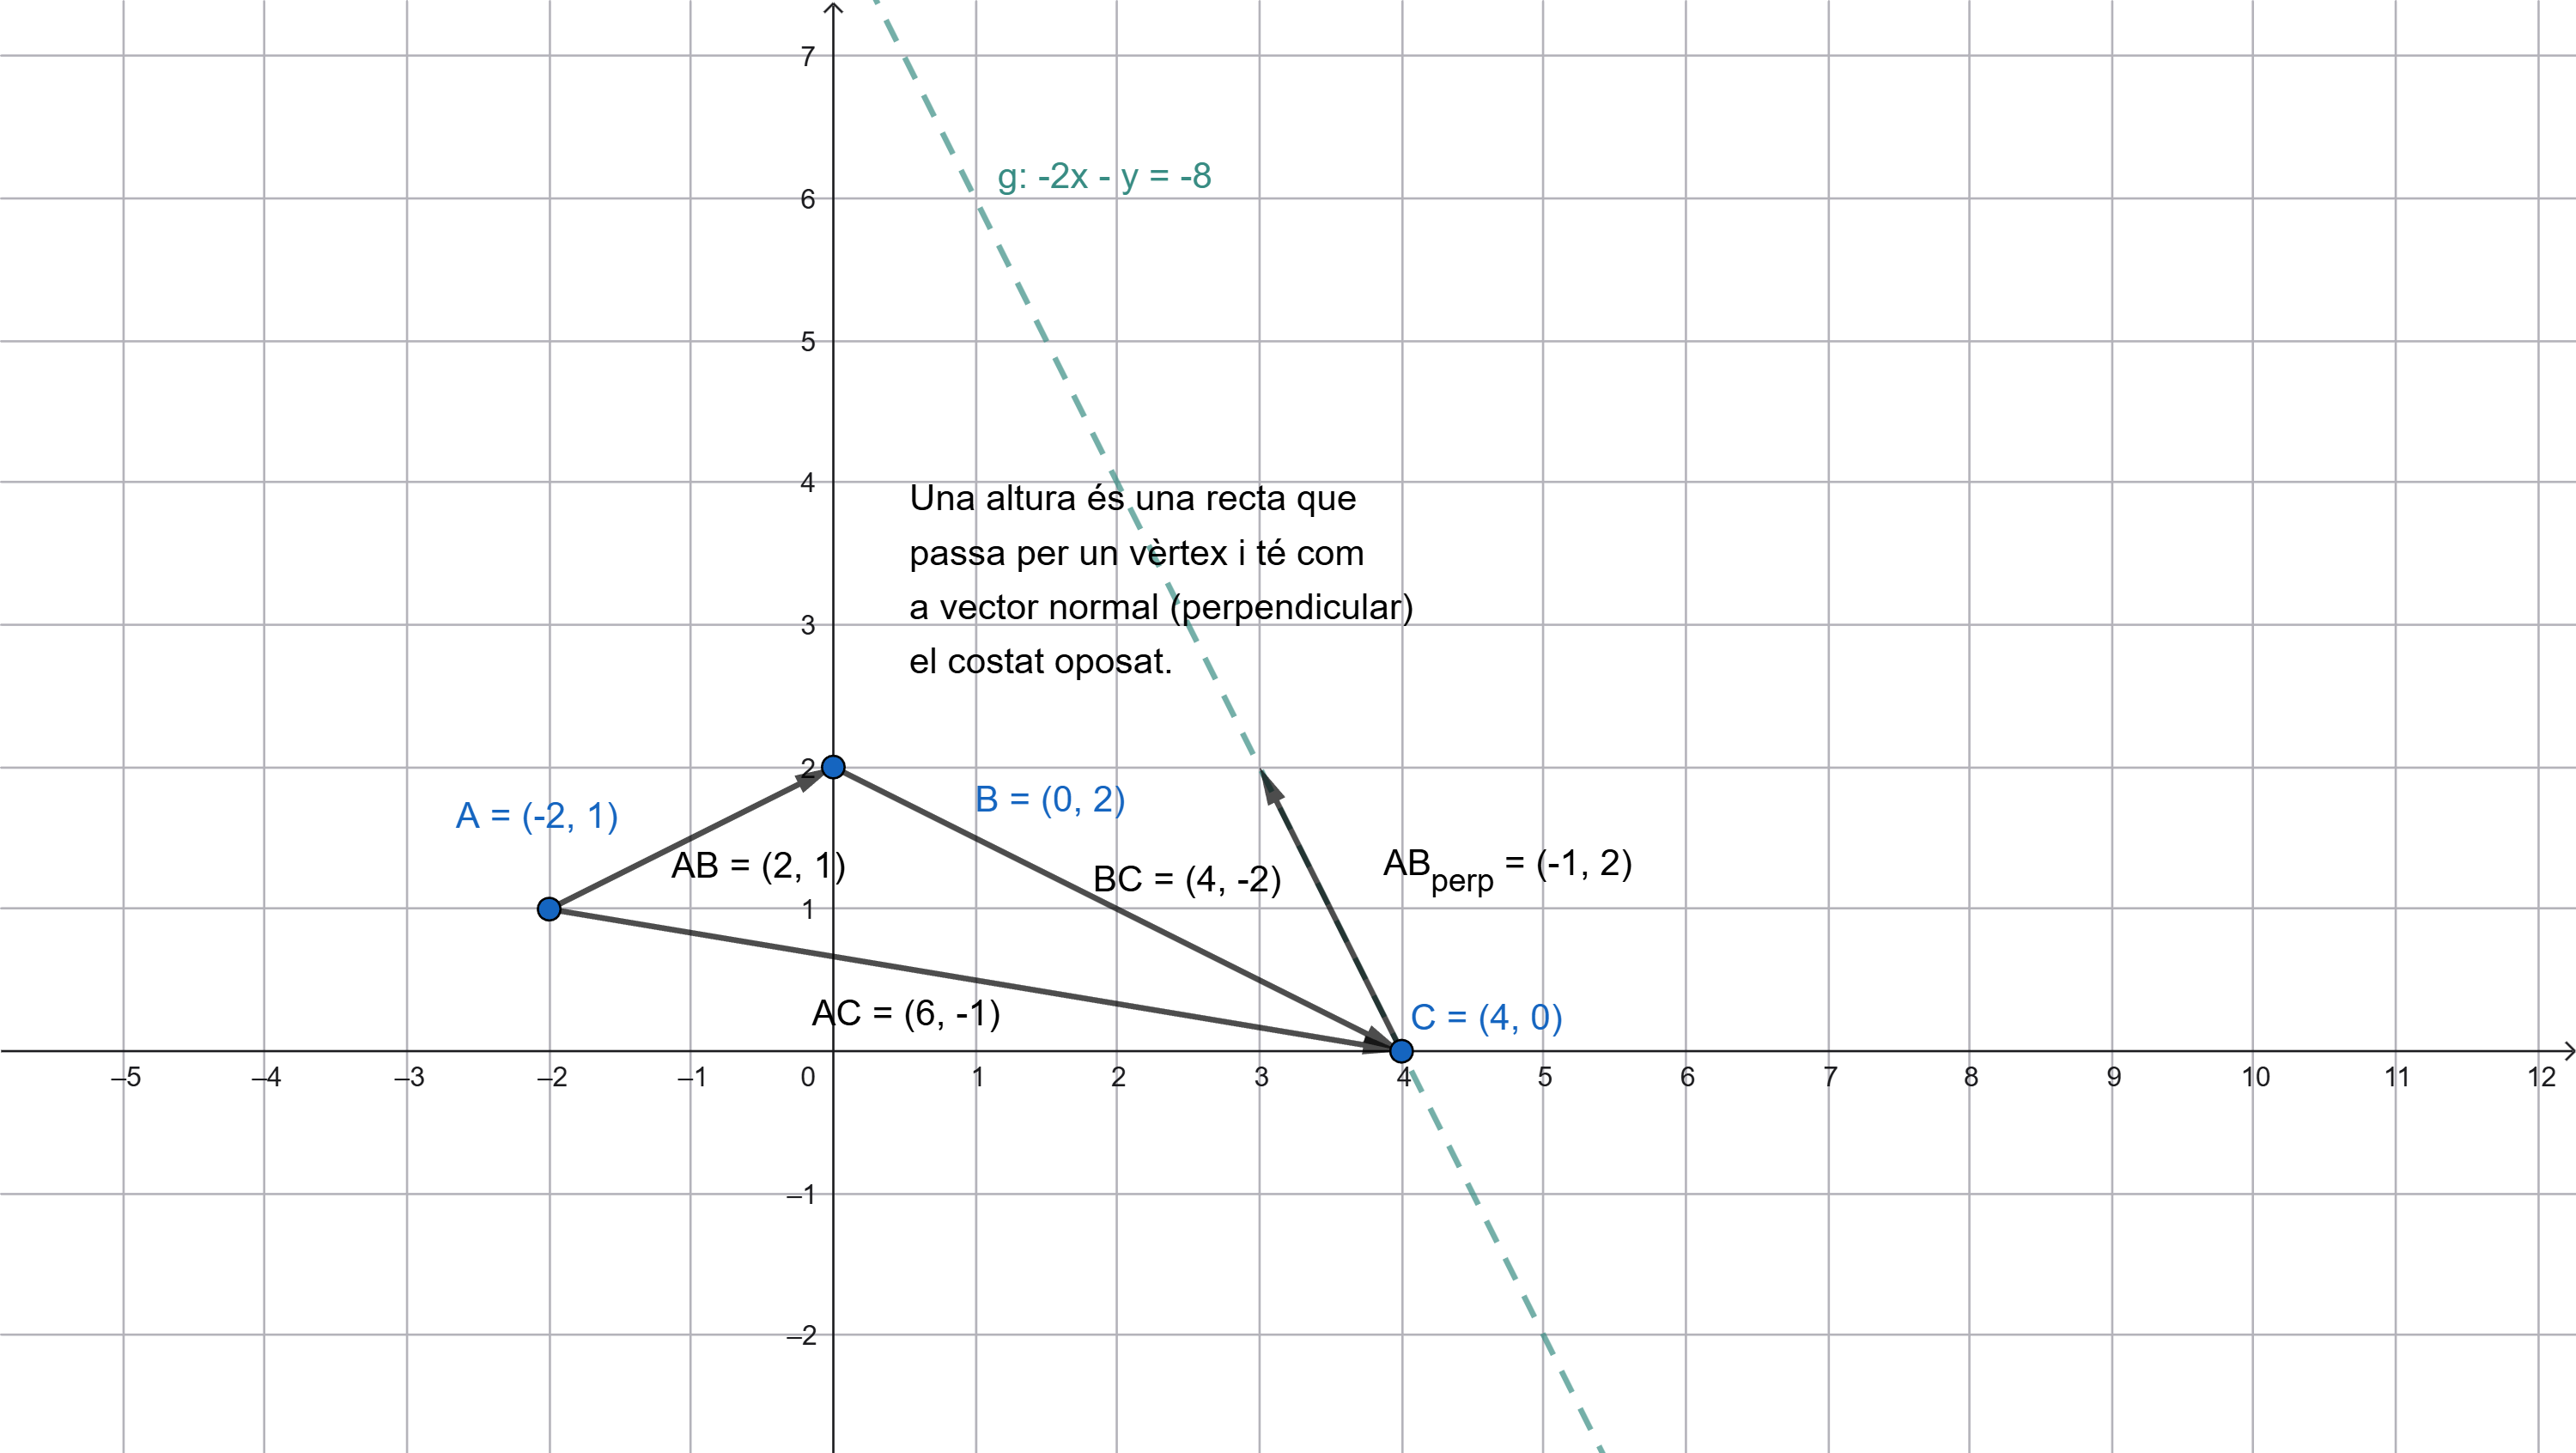
\includegraphics[width=0.7\textwidth]{Rectes - Altures triangle 21 AF_5.png}
    \caption{Representació de l'altura $h_C$.}
\end{figure}

\newpage

% --- Altura h_B ---
\subsection*{3. Altura sobre el vèrtex B ($h_B$)}

L'altura $h_B$ passa pel punt $B(0, 2)$ i és perpendicular al costat $AC$.

\begin{enumerate}
    \item \textbf{Calculem el vector director del costat oposat ($\vec{AC}$):}
    \[ \vec{AC} = C - A = (4, 0) - (-2, 1) = (6, -1) \]
    
    \item \textbf{Identifiquem el vector normal:}
    El vector $\vec{AC}$ és el vector normal ($\vec{n}$) de l'altura $h_B$.
    \[ \vec{n}_{h_B} = (6, -1) \]

    \begin{figure}[H]
        \centering
        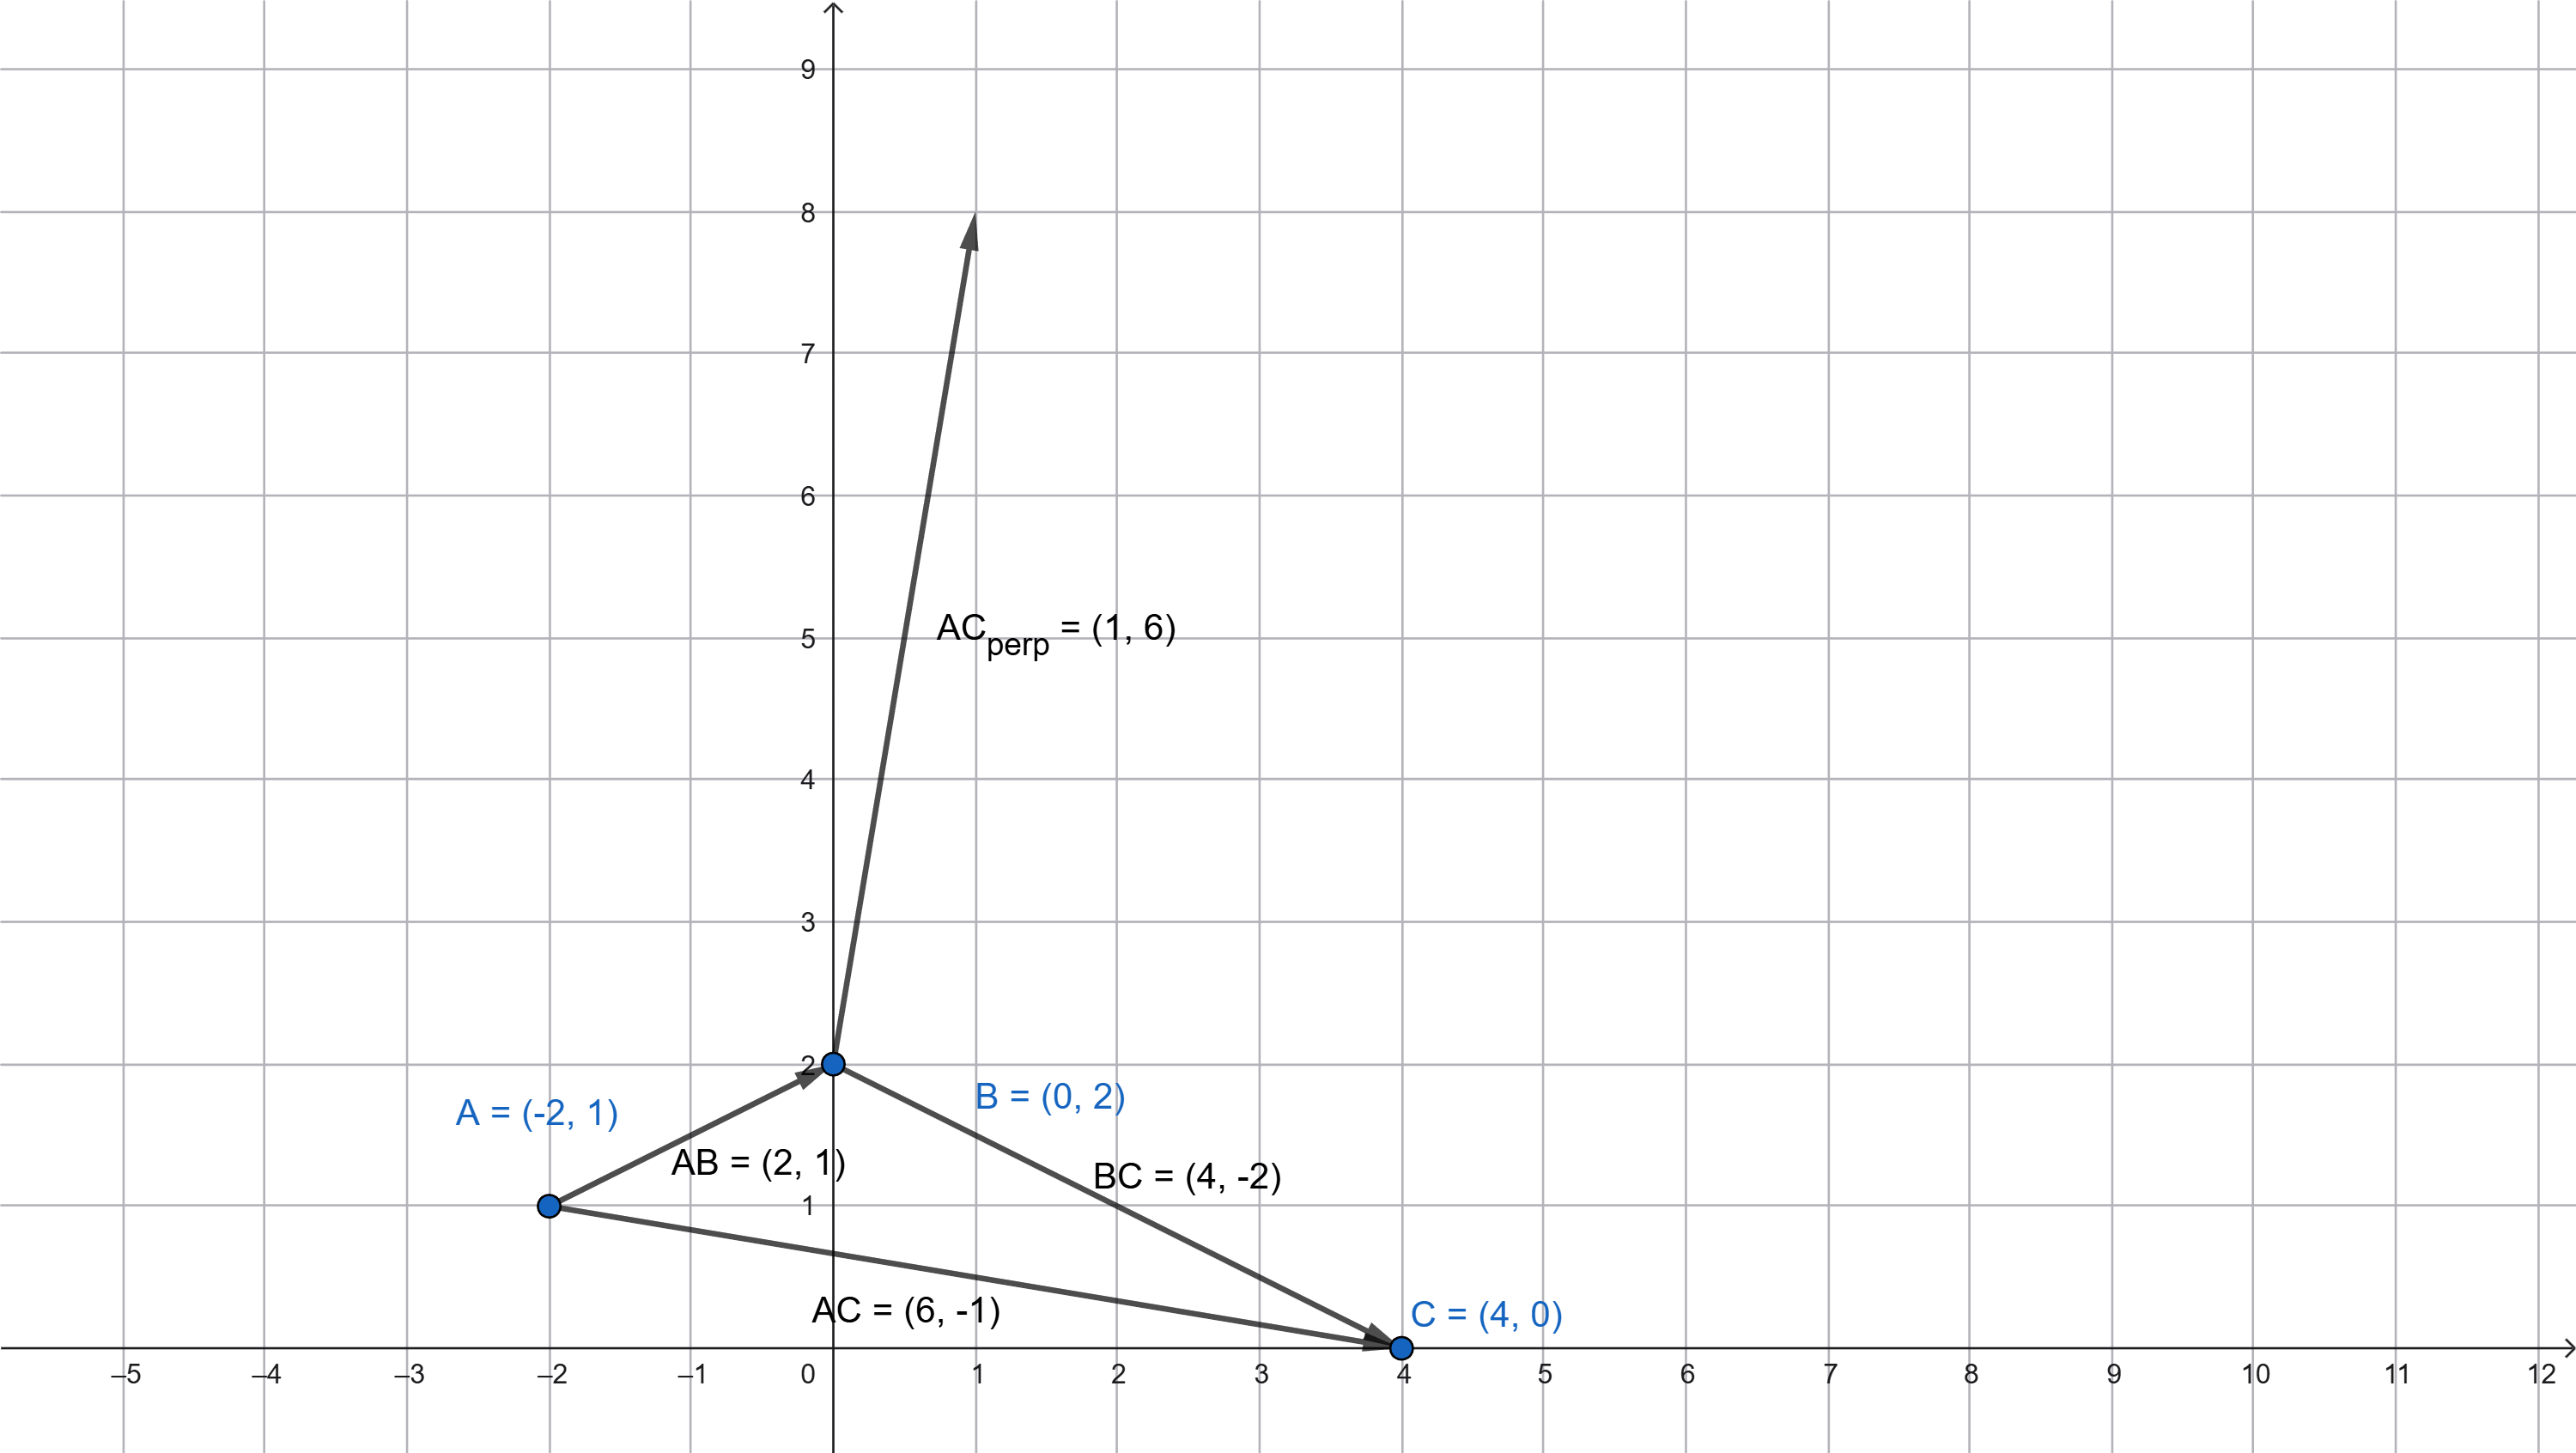
\includegraphics[width=0.7\textwidth]{Rectes - Altures triangle 21 AF_6.png}
        \caption{El vector $\vec{AC}$ és el vector normal per a l'altura des de $B$.}
    \end{figure}

    \item \textbf{Trobem l'equació general:}
    Usant el vector normal $(6, -1)$, l'equació és $6x - y + C = 0$.
    Imposem que passi pel vèrtex $B(0, 2)$:
    \[ 6(0) - 2 + C = 0 \]
    \[ -2 + C = 0 \Rightarrow C = 2 \]
    
    \textbf{L'equació de l'altura $h_B$ és:}
    \[ \boxed{6x - y + 2 = 0} \]
\end{enumerate}

\begin{figure}[H]
    \centering
    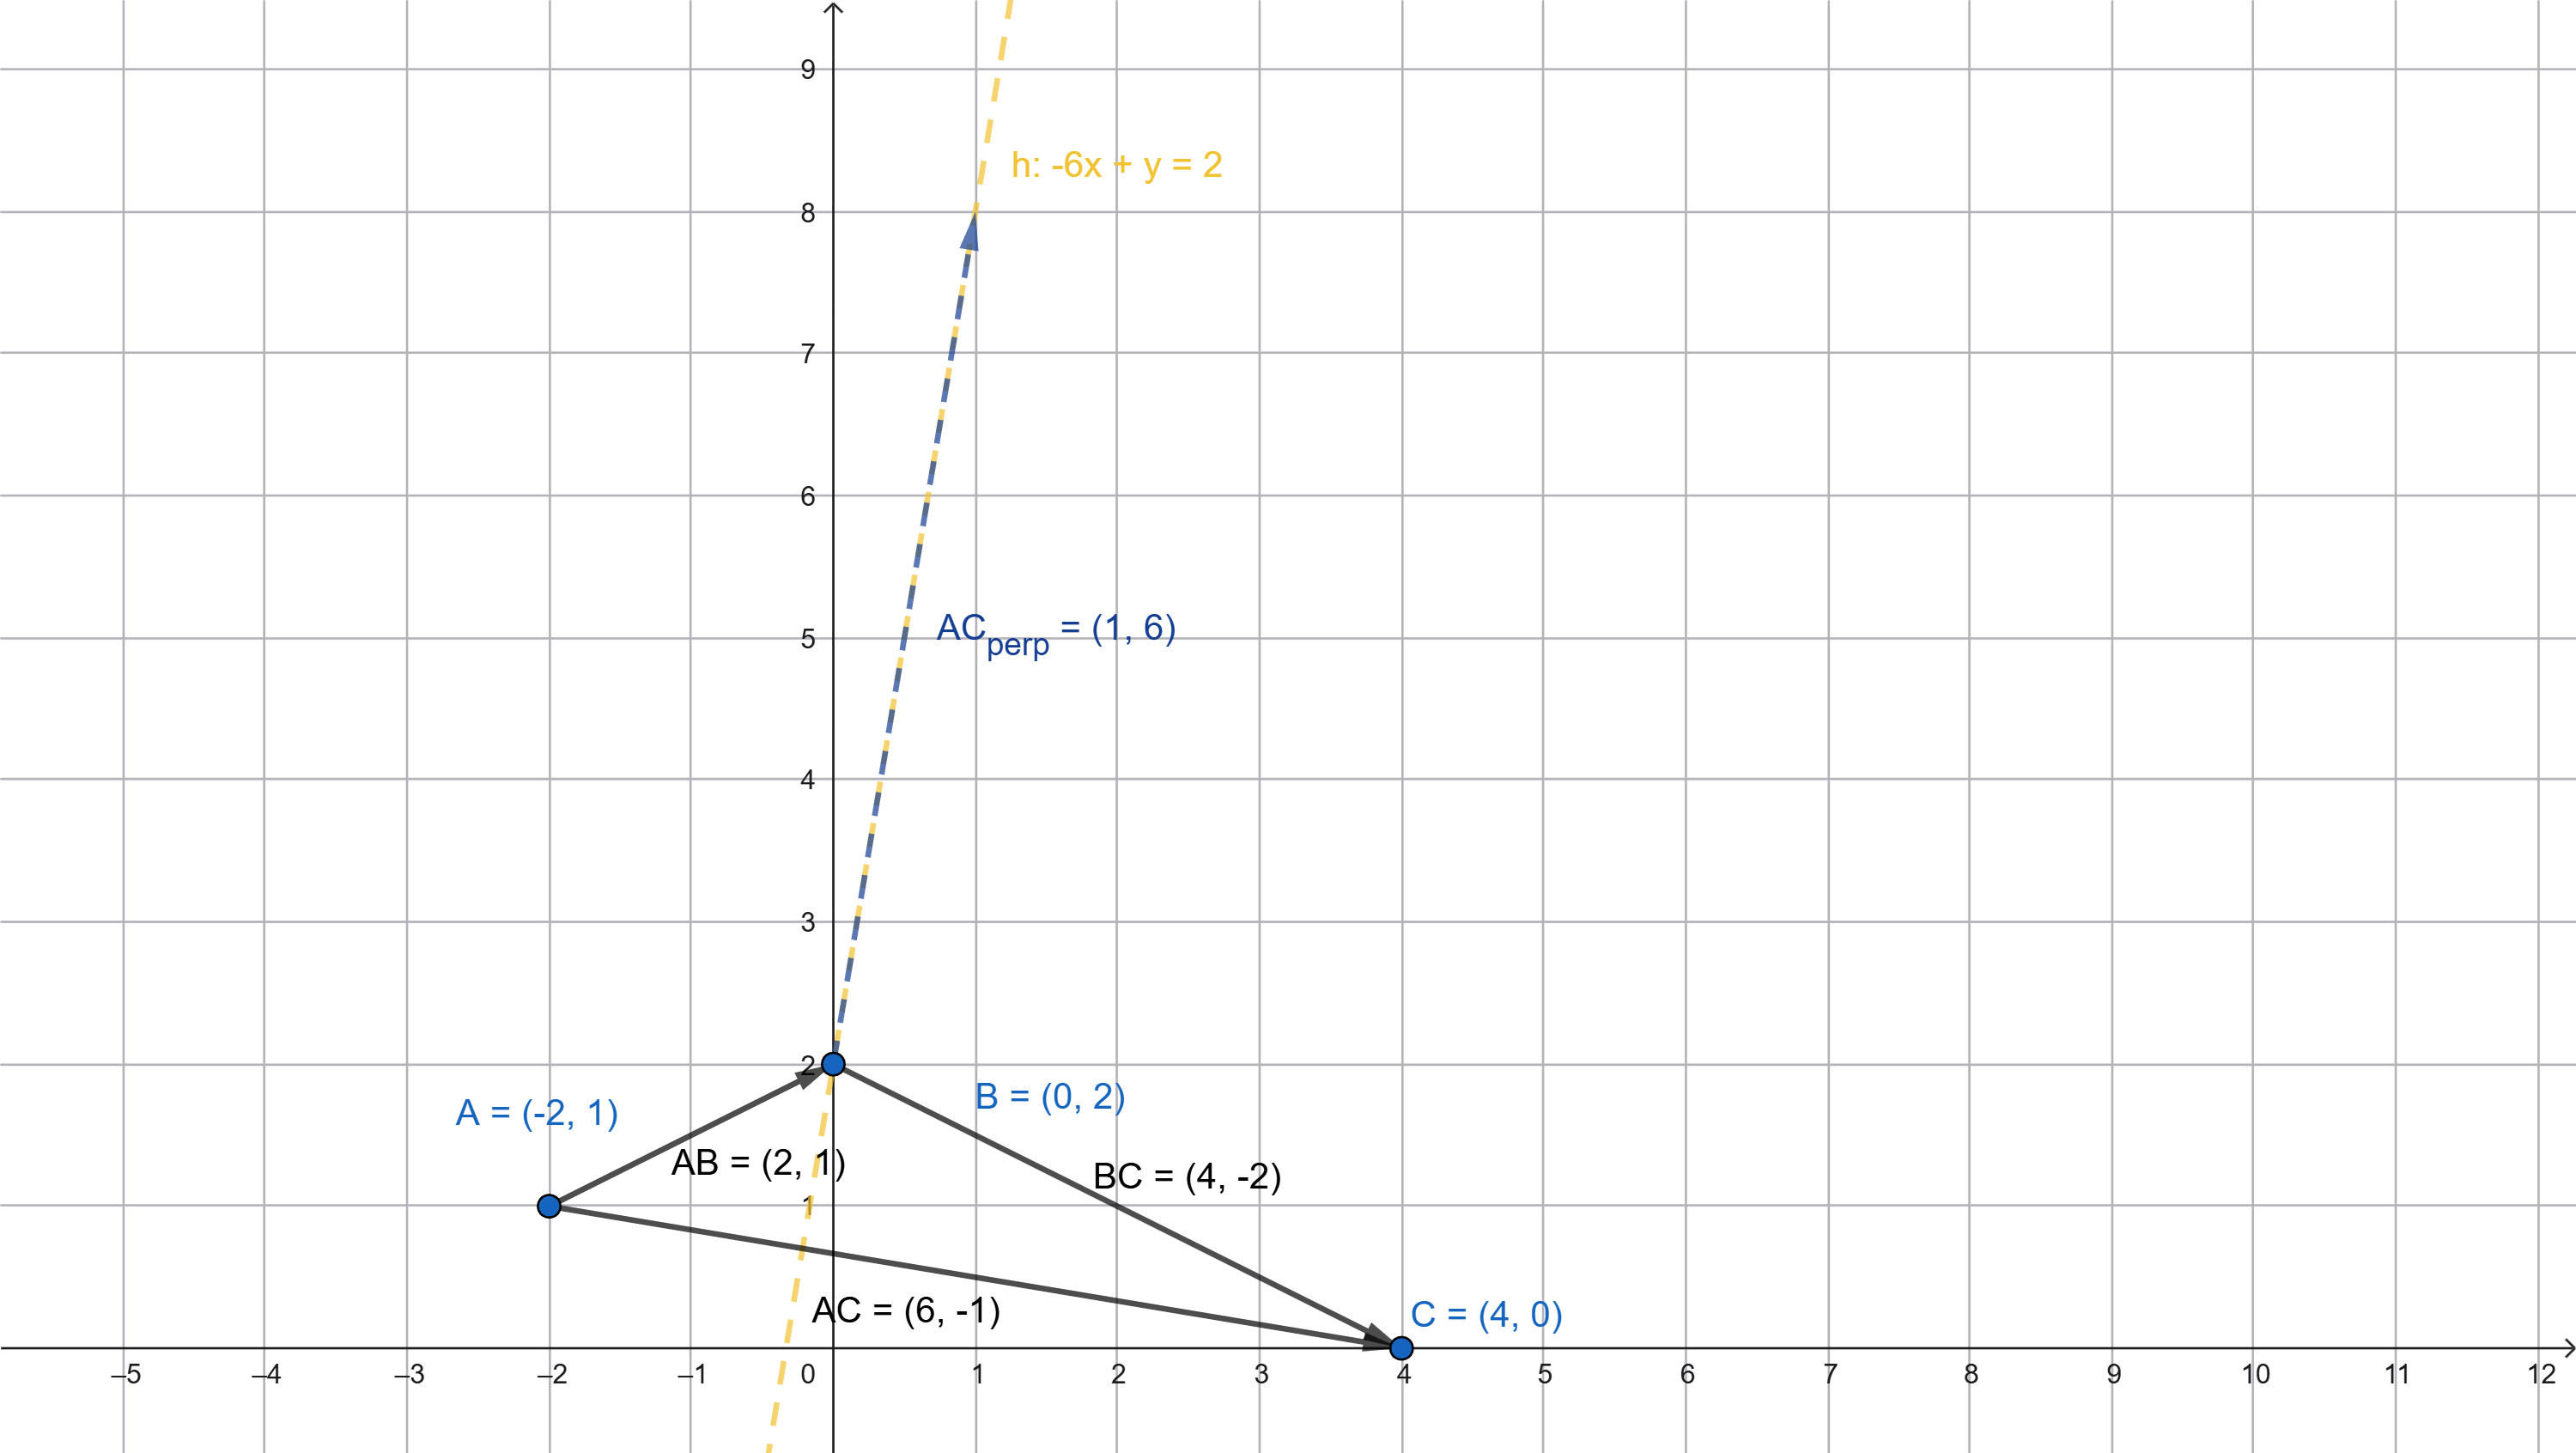
\includegraphics[width=0.7\textwidth]{Rectes - Altures triangle 21 AF_7.png}
    \caption{Representació final amb totes les altures i l'ortocentre.}
\end{figure}




\end{document}